% Created 2014-09-07 So 11:04
\documentclass[presentation]{beamer}
\usepackage[utf8]{inputenc}
\usepackage[T1]{fontenc}
\usepackage{fixltx2e}
\usepackage{graphicx}
\usepackage{longtable}
\usepackage{float}
\usepackage{wrapfig}
\usepackage{rotating}
\usepackage[normalem]{ulem}
\usepackage{amsmath}
\usepackage{textcomp}
\usepackage{marvosym}
\usepackage{wasysym}
\usepackage{amssymb}
\usepackage{hyperref}
\tolerance=1000
\renewcommand{\maketitle}{\begin{frame}\begin{center}\Large
\vspace{1.5cm}
Nuclear Disarmament - Hacks\\ for a world free of nuclear weapons?\\[0.5em]\small\insertauthor\\[1em]\tiny moritz@nuclearfreesoftware.org\\[1em]
MRMCD, \insertdate\\[0.5em]
\vspace{1.8cm} 
\includegraphics[width=1.5cm]{by-nc-sa_eu.png}\\\fontsize{5pt}{6}\selectfont \textcolor{gray!85}{This work is licensed under the\\ Creative Commons Attribution-NonCommercial-ShareAlike 4.0 International License.\\ To view a copy of this license, visit http://creativecommons.org/licenses/by-sa/4.0/.}
\end{center}\end{frame}}
\usepackage{ctable}
\usepackage{tabularx}
\usepackage{animate}
\usepackage{listings}
\usepackage{ulem}
\makeatletter
\def\s@out@end{\relax\relax\relax}
\def\s@out#1\s@out@end{\sout{#1}}
\def\makestrikeout<#1>#2{\only<#1>{\s@out}#2\s@out@end}
\makeatletter
\newbox\@backgroundblock
\newenvironment{backgroundblock}[2]{%
\global\setbox\@backgroundblock=\vbox\bgroup%
\unvbox\@backgroundblock%
\vbox to0pt\bgroup\vskip#2\hbox to0pt\bgroup\hskip#1\relax%
}{\egroup\egroup\egroup}
\addtobeamertemplate{background}{\box\@backgroundblock}{}
\makeatother
\newcolumntype{L}{>{\raggedright\let\newline\\\arraybackslash\hspace{0pt}}X}
\newcolumntype{R}{>{\raggedleft\let\newline\\\arraybackslash\hspace{0pt}}X}
\newcommand\imagesource[1]{\tiny #1}
\newenvironment{newcolbox}[2]{\begin{tcolorbox}[tcbeamer,notitle,colback=#1,colupper=black] \includegraphics[width=\textwidth]{people/#2.png}\centering\tiny}{\end{tcolorbox}\vskip}
\usetheme{DarkBeamer}
\author{Moritz Kütt}
\date{September 2014}
\title{Nuclear Disarmament - Hacks for a world free of nuclear weapons?}
\hypersetup{
  pdfkeywords={},
  pdfsubject={},
  pdfcreator={Emacs 24.3.1 (Org mode 8.2.7b)}}
\begin{document}

\maketitle

\section{Nuclear Weapons 101}
\label{sec-1}
\begin{frame}[label=sec-1-1]{}
\begin{center}
\makestrikeout<2>{How to build a nuclear weapon?}\\[1em]
\only<2>{What do we need to know to disarm a nuclear weapon?}
\end{center}
\end{frame}

\begin{frame}[label=sec-1-2]{Basic principle}
\begin{columns}
\begin{column}{0.45\textwidth}
Energy produced by reactions of atomic nucleus.

\begin{varblock}[\textwidth]{}

\includegraphics[width=0.1\textwidth]{images/proton} ~ Proton \\[0.5em]

\includegraphics[width=0.1\textwidth]{images/neutron} ~ Neutron
\end{varblock}

\footnotesize

\begin{description}
\item[{Elements}] Depend on proton number
\item[{Isotopes}] Different neutron numbers for particular proton number
\end{description}
\end{column}

\begin{column}{0.45\textwidth}

Fission of heavy elements produces large amount of energy:

\begin{varblock}[\textwidth]{}
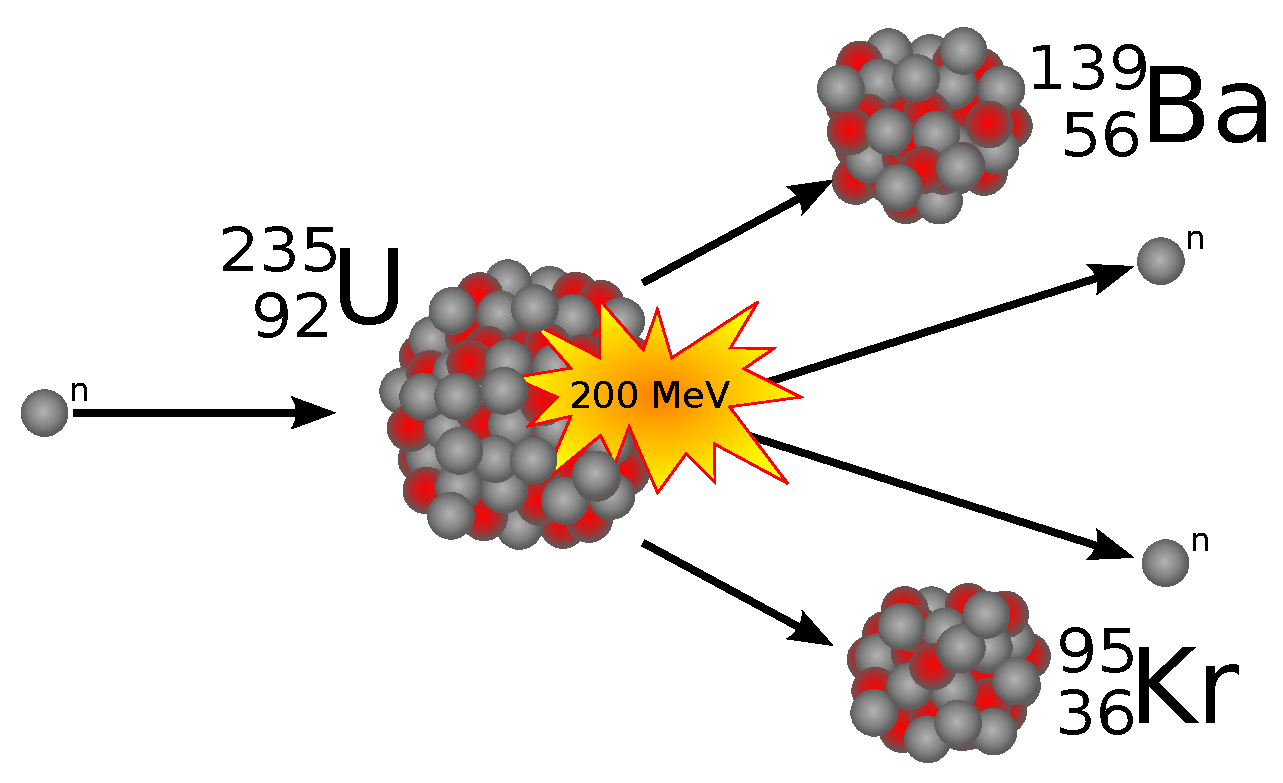
\includegraphics[width=0.95\textwidth]{images/Kernspaltung}
\end{varblock}
\vspace{-0.4cm}
 \tiny \textcolor{gray}{CC-BY-SA - Stefan-Xp}

\normalsize
    C-oxidation: several eV
\end{column}
\end{columns}
\end{frame}




\begin{frame}[label=sec-1-3]{Nuclear Chain Reaction}
\begin{columns}
\begin{column}{0.45\textwidth}

Initial fission leading to exponential growth of fissions.

\begin{block}{Critical Mass}
Minimal amount of material needed for which chain reaction is possible.\\
\end{block}

Smaller amount: more neutrons lost by absorption / escape.
\end{column}

\begin{column}{0.45\textwidth}

\begin{varblock}[0.9 \textwidth]{}
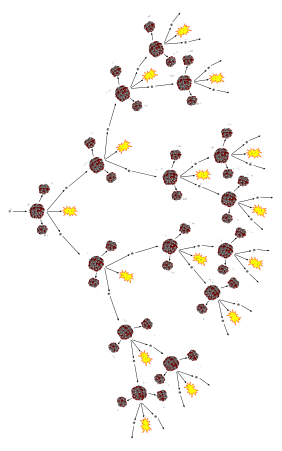
\includegraphics[width=\textwidth]{images/Kettenreaktion}
\end{varblock}

\begin{tikzpicture}[remember picture, overlay]
\node [shift={(5.5cm, -2.2cm)},rotate = 90] at (current page.center) {\tiny \textcolor{gray}{CC-BY-SA - Wikimedia Commons}};
\end{tikzpicture}
\end{column}
\end{columns}
\end{frame}

\begin{frame}[label=sec-1-4]{Fissile Material}
\begin{center}
for weapon purposes do not occur naturally
\end{center}

\begin{columns}[t]
\begin{column}{0.5\textwidth}
\begin{block}{Highly Enriched Uranium}
\small
Protons: 92\\
    Neutrons: 235/238\\[1em]

Natural uranium: 0.7\% U-235\\
    For weapons: $>$ 90\% U-235 needed\\[0.5em]

U-235 fraction can be increased by \alert{enrichment}.\\[0.8em]

\textcolor{gray}{Highly Enriched Uranium =  HEU}
\end{block}
\end{column}


\begin{column}{0.45\textwidth}
\begin{block}{Plutonium}
\small Protons: 94\\
    Neutrons: 239 (240/241/\ldots{})\\[1em]


Plutonium produced in any nuclear reactor.\\[0.5em]

It needs to be separated from spent fuel by \alert{reprocessing}.
\end{block}
\end{column}
\end{columns}
\end{frame}

\begin{frame}[label=sec-1-5]{Weapon Principles}
\vspace{-0.7cm}
\begin{columns}[t]
\begin{column}{0.45\textwidth}
\begin{block}{Gun Type}

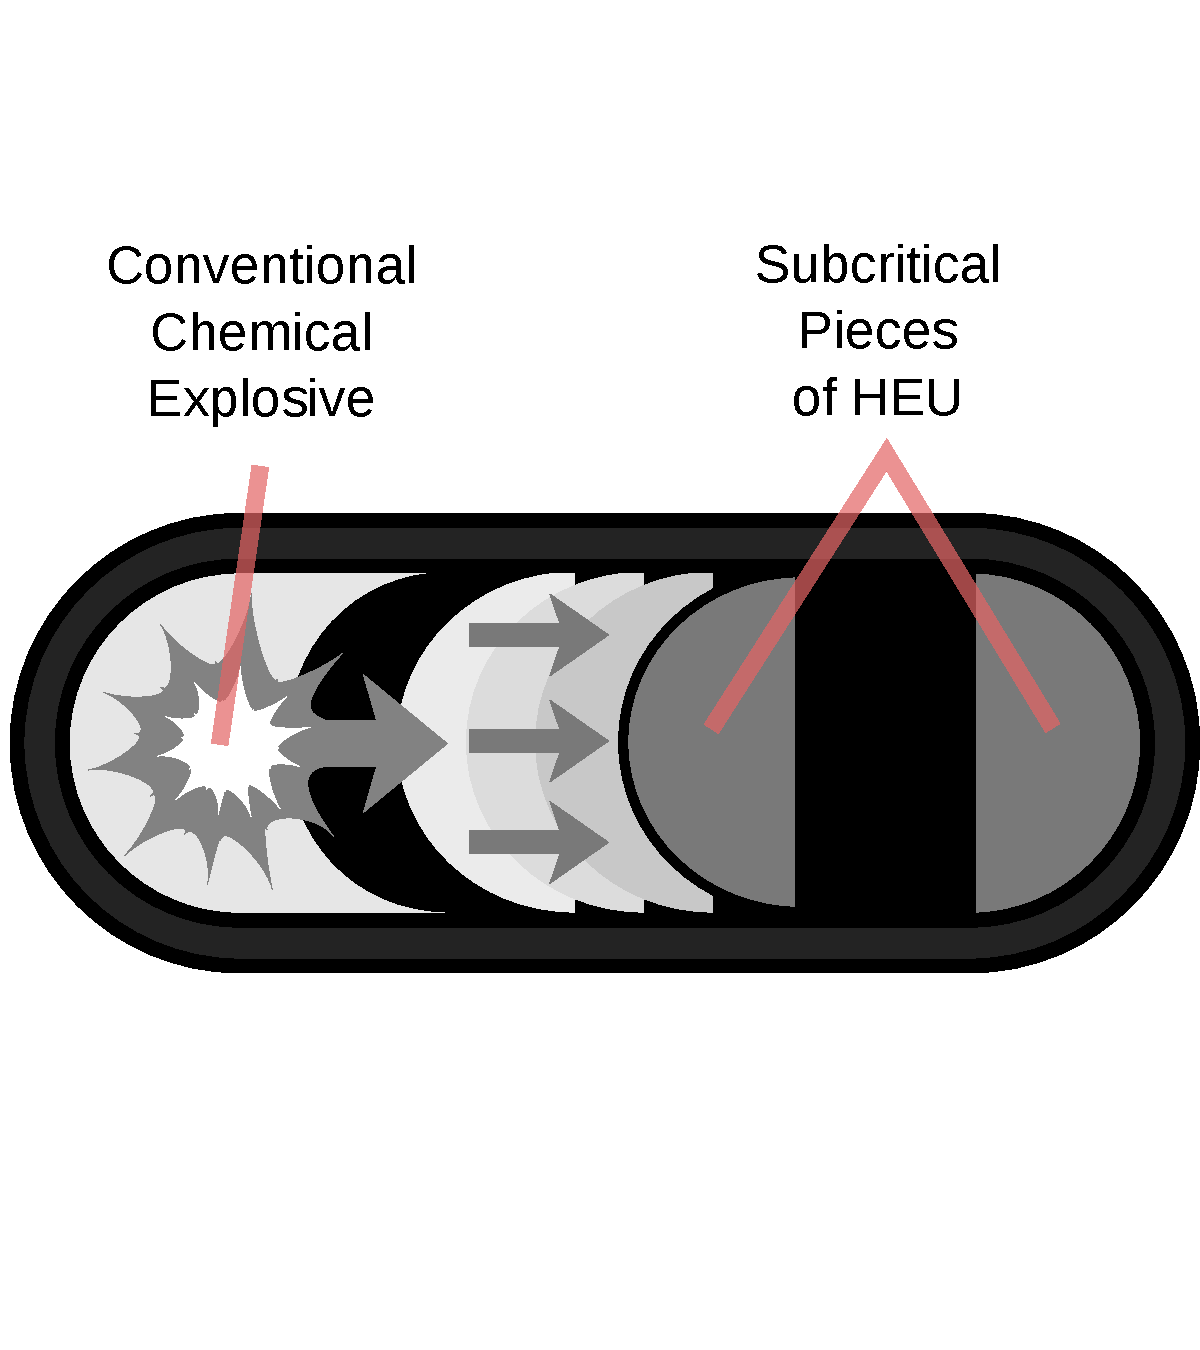
\includegraphics[width=\textwidth]{images/guntype_modified}
\end{block}
\end{column}

\begin{column}{0.45\textwidth}
\begin{block}{Implosion}
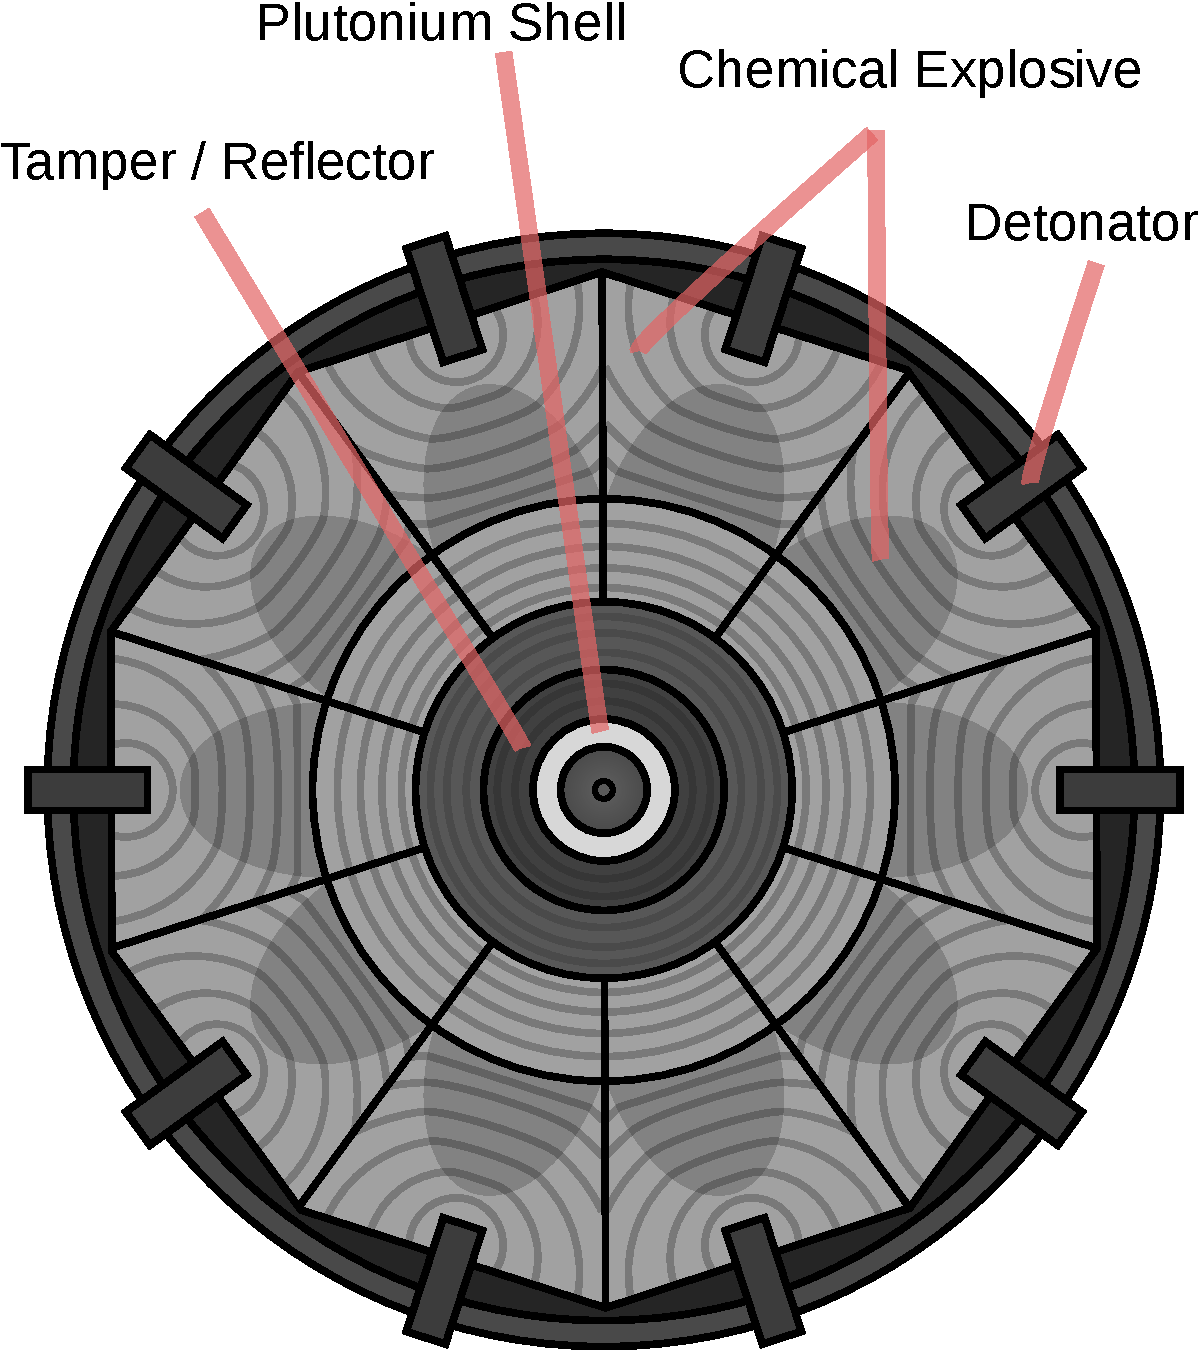
\includegraphics[width=\textwidth]{images/implosion_modified}
\end{block}
\end{column}
\end{columns}

\begin{columns}
\begin{column}{0.45\textwidth}
\tiny \textcolor{gray}{Public Domain - Wikimedia Commons (Modified)}
\end{column}

\begin{column}{0.45\textwidth}
\tiny \textcolor{gray}{Public Domain - Wikimedia Commons (Modified)}
\end{column}
\end{columns}
\end{frame}


\begin{frame}[label=sec-1-6]{Massive Explosive Power}
\begin{columns}
\begin{column}{0.58\textwidth}
\vspace{-0.5cm}
\begin{center}
Approx. 2000 nuclear weapons were exploded during nuclear testing.\\[1em]

Total yield (explosive power) of all tested weapons: \\
510 million tons TNT equivalent

\fontsize{3pt}{3.6}\selectfont \textcolor{gray}{R.S. Norris and W.M. Arkin, NRDC Nuclear Notebook - Known Nuclear Tests Worldwide, 1945--1998, \emph{Bulletin of the Atomic Scientists}, 1998, 1, 2003}\\[1em]

\normalsize

\pause
Can you imagine\\ 510.000.000.000 kg \\ of TNT?\\[1em]

\pause

\end{center}
\end{column}

\begin{column}{0.38\textwidth}

\vspace{-0.8cm}

\begin{center}
1.000 kg did this...
\end{center}

\vspace{-0.85cm}

\begin{varblock}[0.95\textwidth]{}
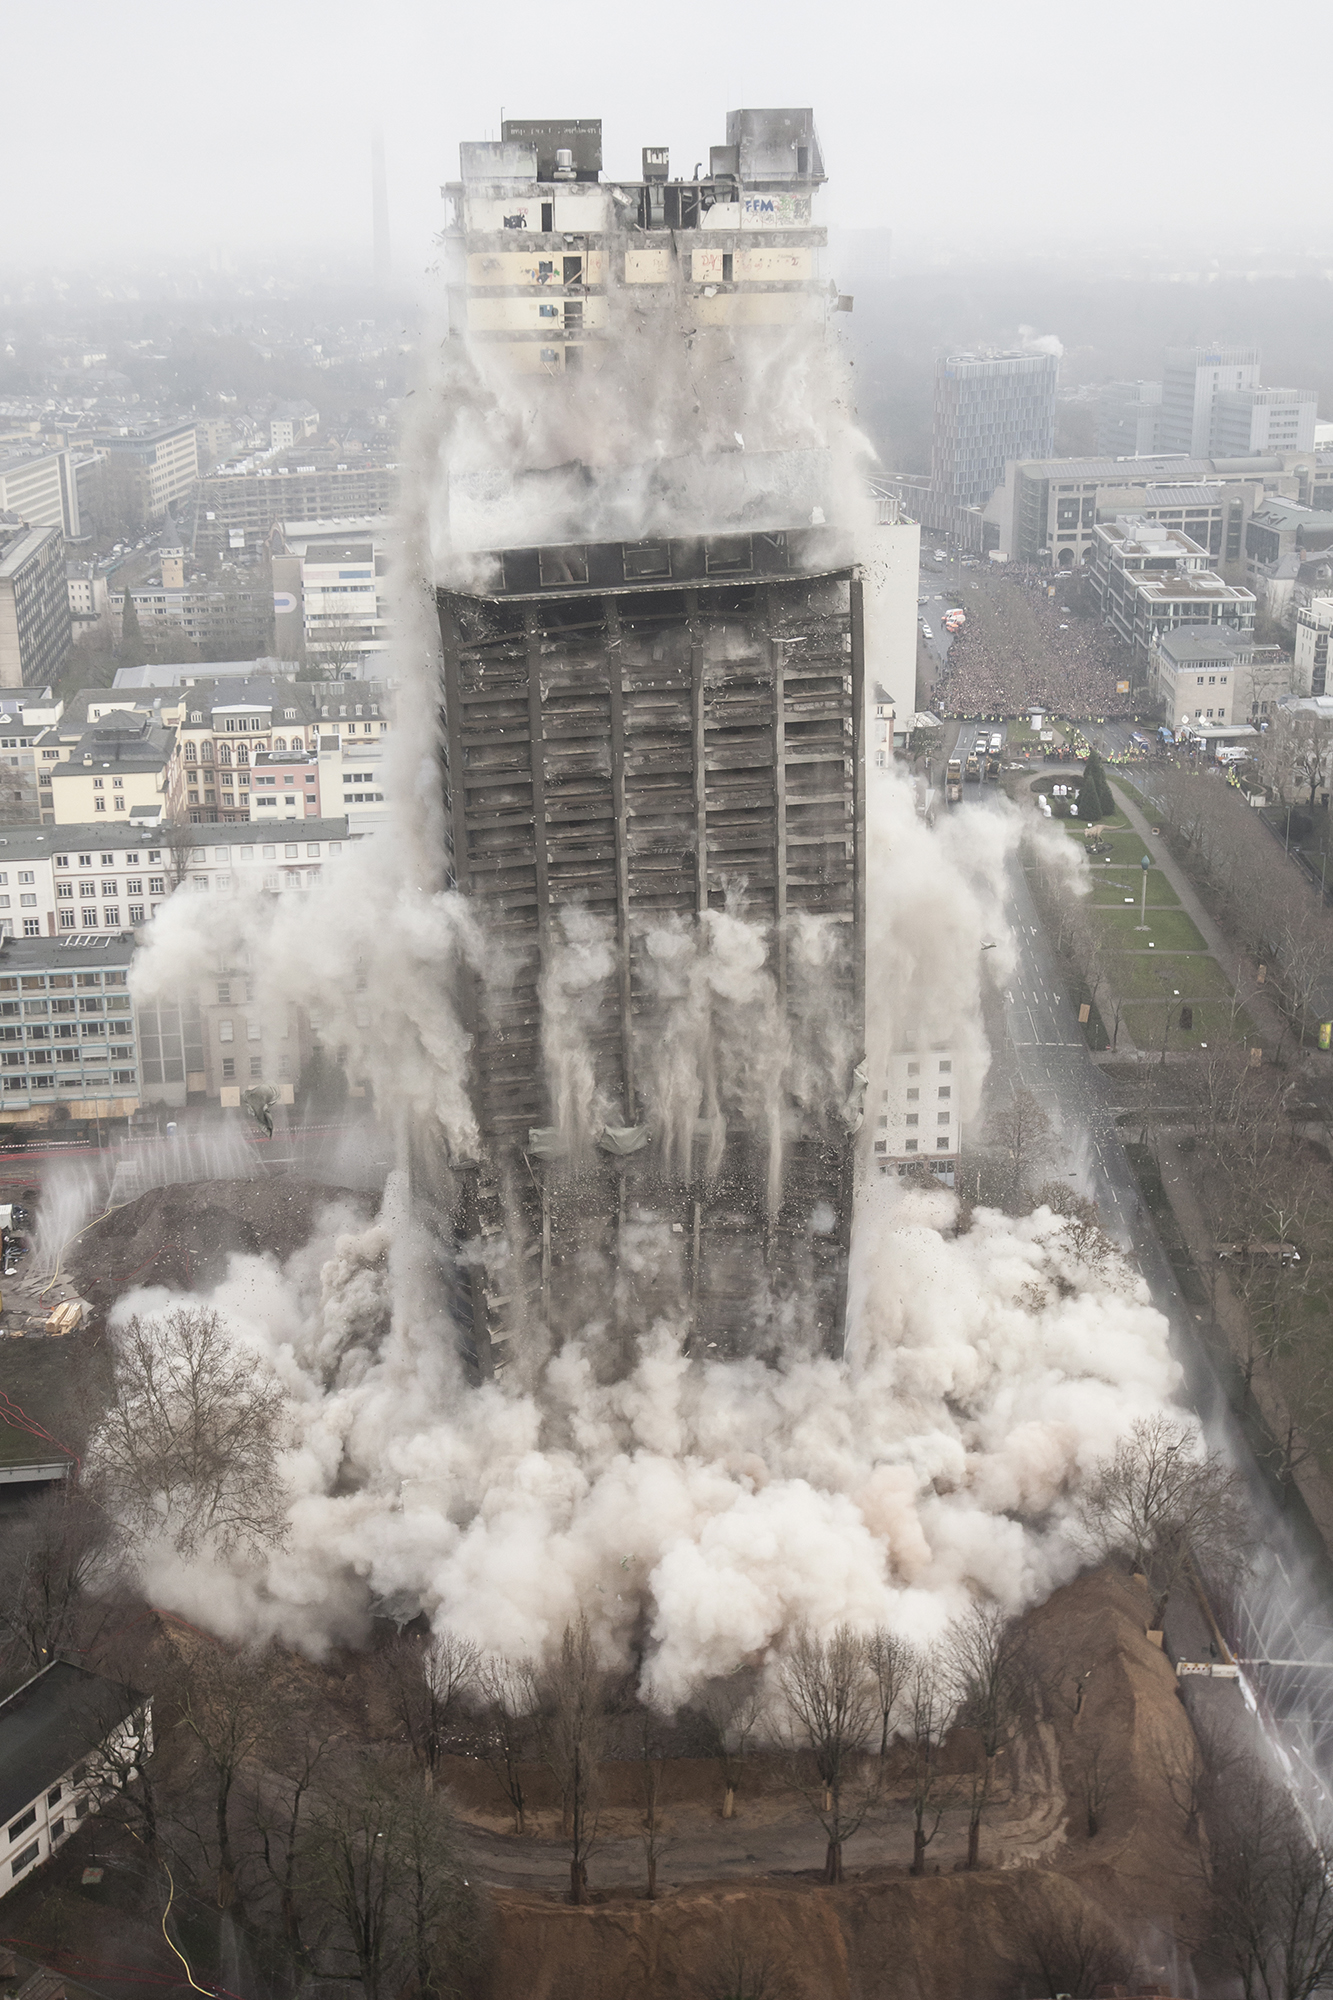
\includegraphics[width=\textwidth]{images/140202_Afe-Tower_Blasting.jpg}
\end{varblock}
\vspace{-0.3cm}
\tiny \textcolor{gray}{CC-BY-SA Sajak}
\end{column}
\end{columns}
\end{frame}

\begin{frame}[label=sec-1-7]{}

\begin{backgroundblock}{10mm}{10mm}
%\begin{varblock}[\textwidth]{}
  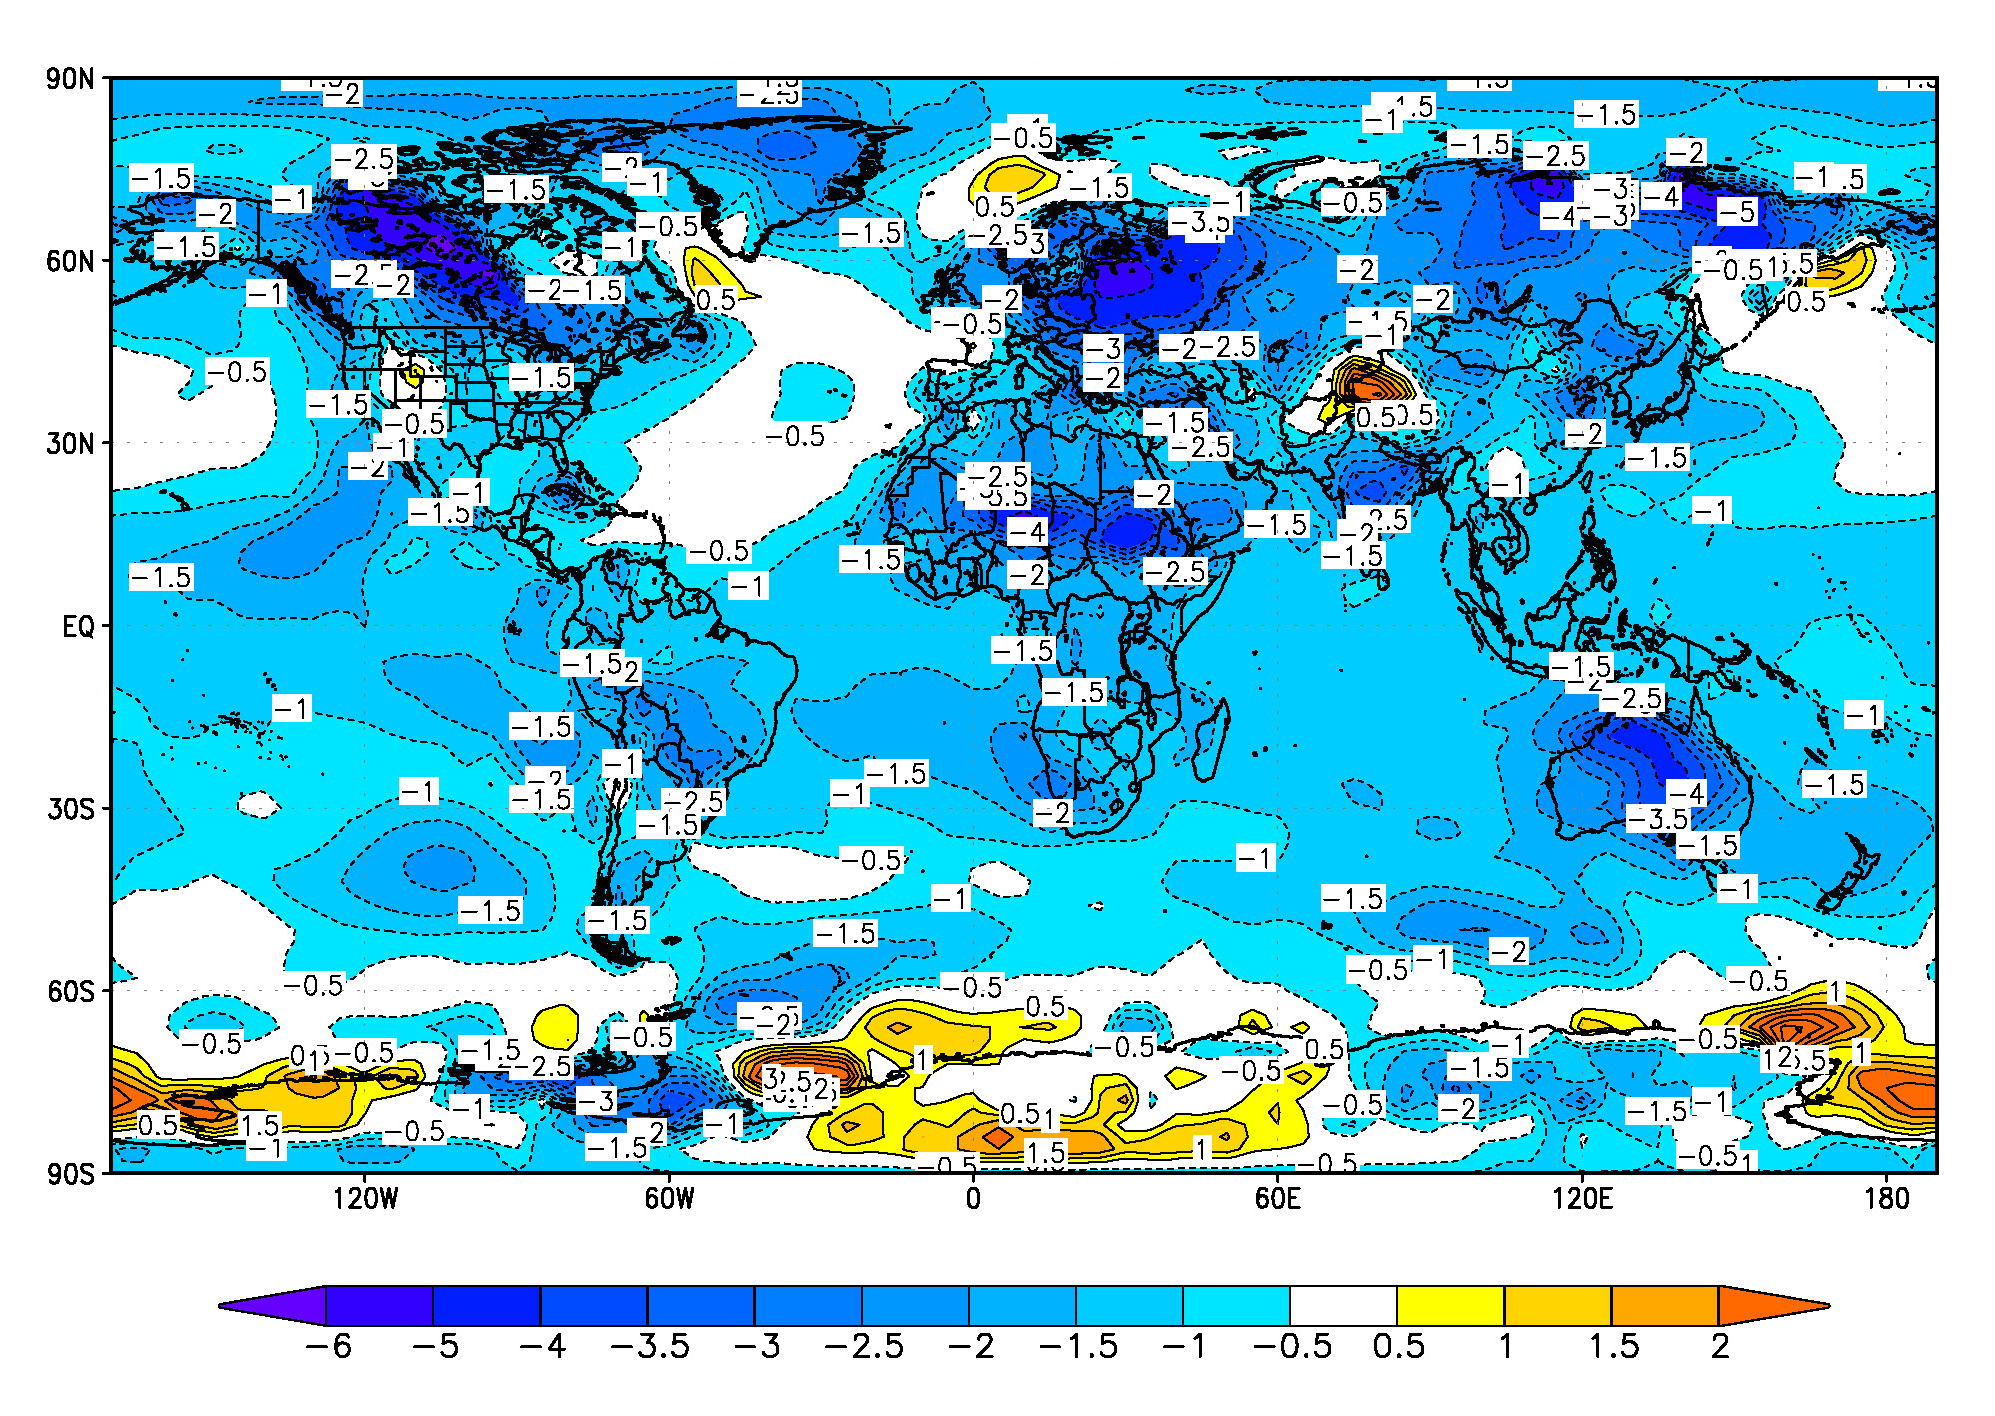
\includegraphics[width=\textwidth]{images/Fig5SummerTempMap_modified.jpg}
%\end{varblock}%
\end{backgroundblock}%


\begin{columns}
\begin{column}{0.6\textwidth}
\vspace{8.3cm}

\hspace{0.5cm} \tiny \textcolor{gray}{CC-BY-SA-NC Robock et. al 2007, Fig. 5}%
\end{column}

\begin{column}{0.4\textwidth}
\vspace{2.5cm}

\begin{block}{Nuclear Winter}
\footnotesize Temperature change resulting from regional nuclear war (100 warheads).
\end{block}
\end{column}
\end{columns}
\end{frame}

\begin{frame}[label=sec-1-8]{Global Warhead stockpiles}
\begin{varblock}[\textwidth]{}
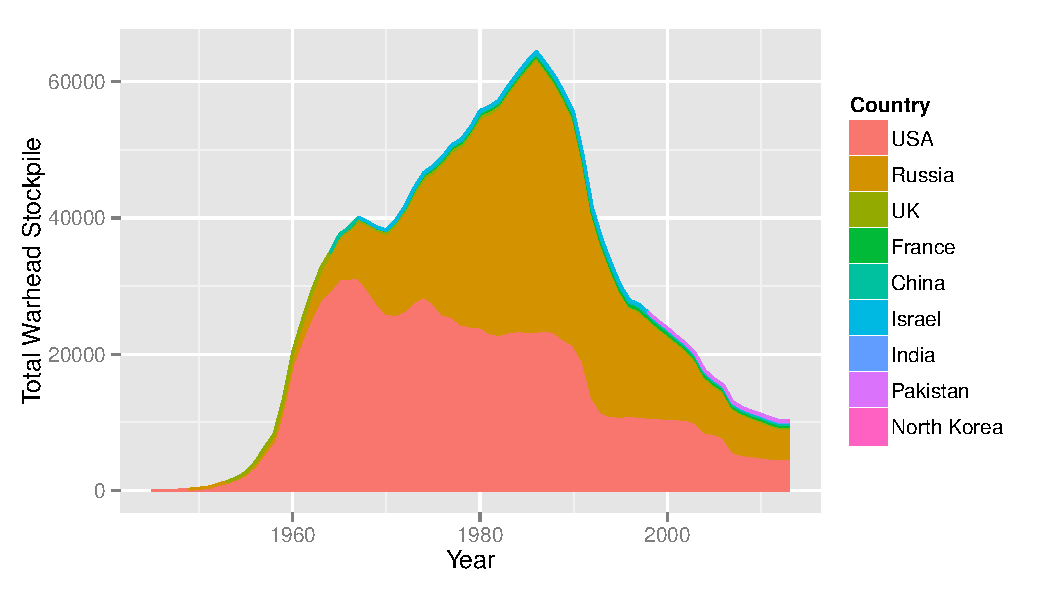
\includegraphics[width=\textwidth]{images/all_countries}
\end{varblock}

\vspace{-0.4cm}
\fontsize{3pt}{3.6}\selectfont \textcolor{gray}{Image created with data from: Kristensen, H. M. and Norris, R. S. Global nuclear weapons inventories, 1945-2013 Bulletin of the Atomic Scientists, SAGE Publications, 2013, 69, 75–81}

\normalsize
\end{frame}

\begin{frame}[label=sec-1-9]{Germany}
\vspace{-0.5cm}
\begin{center}
Nuclear Weapons in Germany?\\[0.7em]
\pause
U.S. nuclear weapons stationed as part of "NATO nuclear sharing"
\end{center}

\vspace{-0.3cm}
\begin{columns}[t]
\begin{column}{0.48\textwidth}
\begin{block}{approx. 20 stored at Büchel}
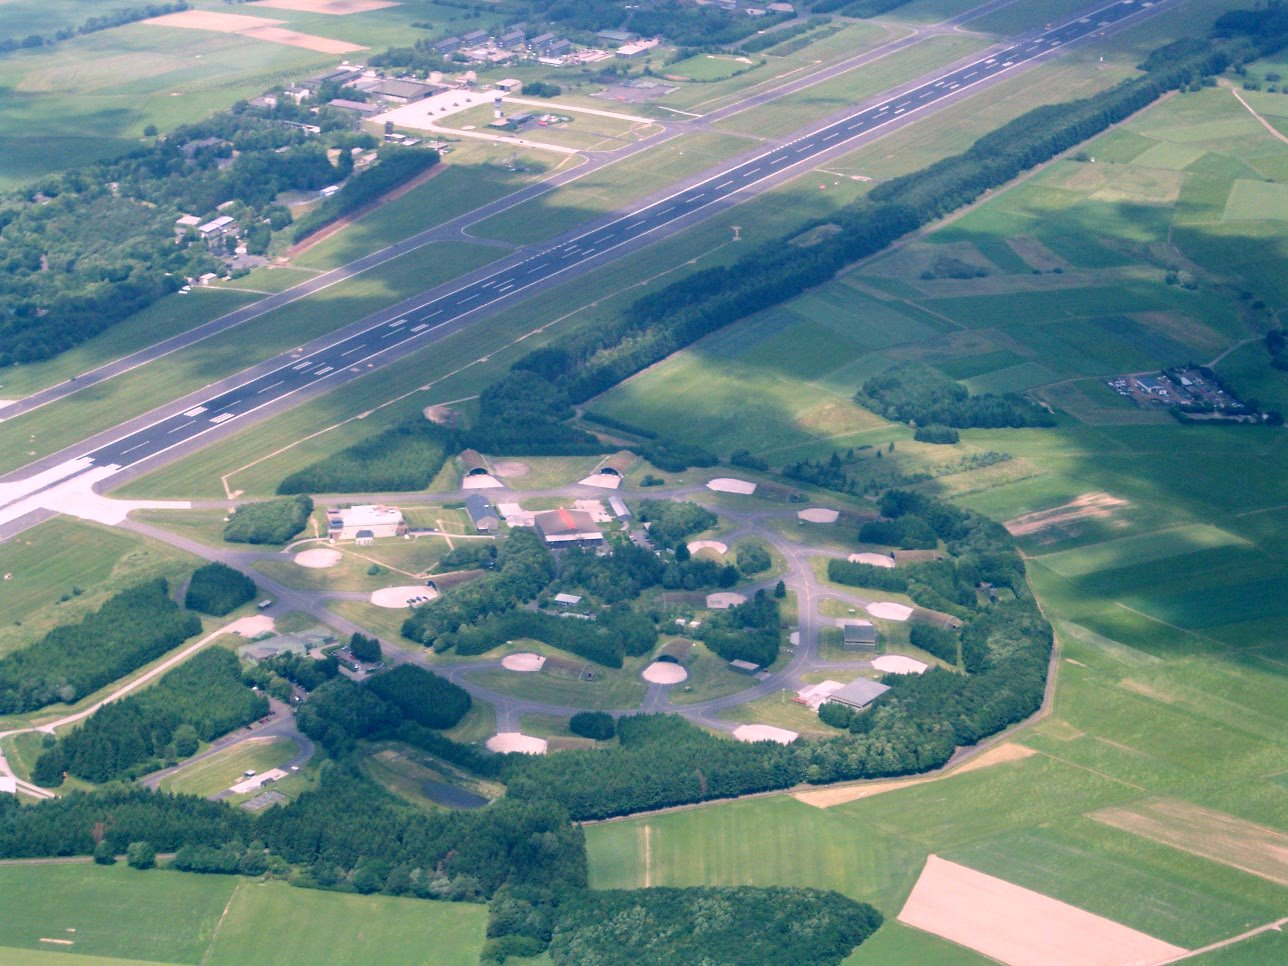
\includegraphics[width=\textwidth]{images/Buechel_Fliegerhorst.jpg}
\end{block}
\end{column}

\begin{column}{0.48\textwidth}
\begin{block}{B61 warheads}

\vspace{0.2cm}

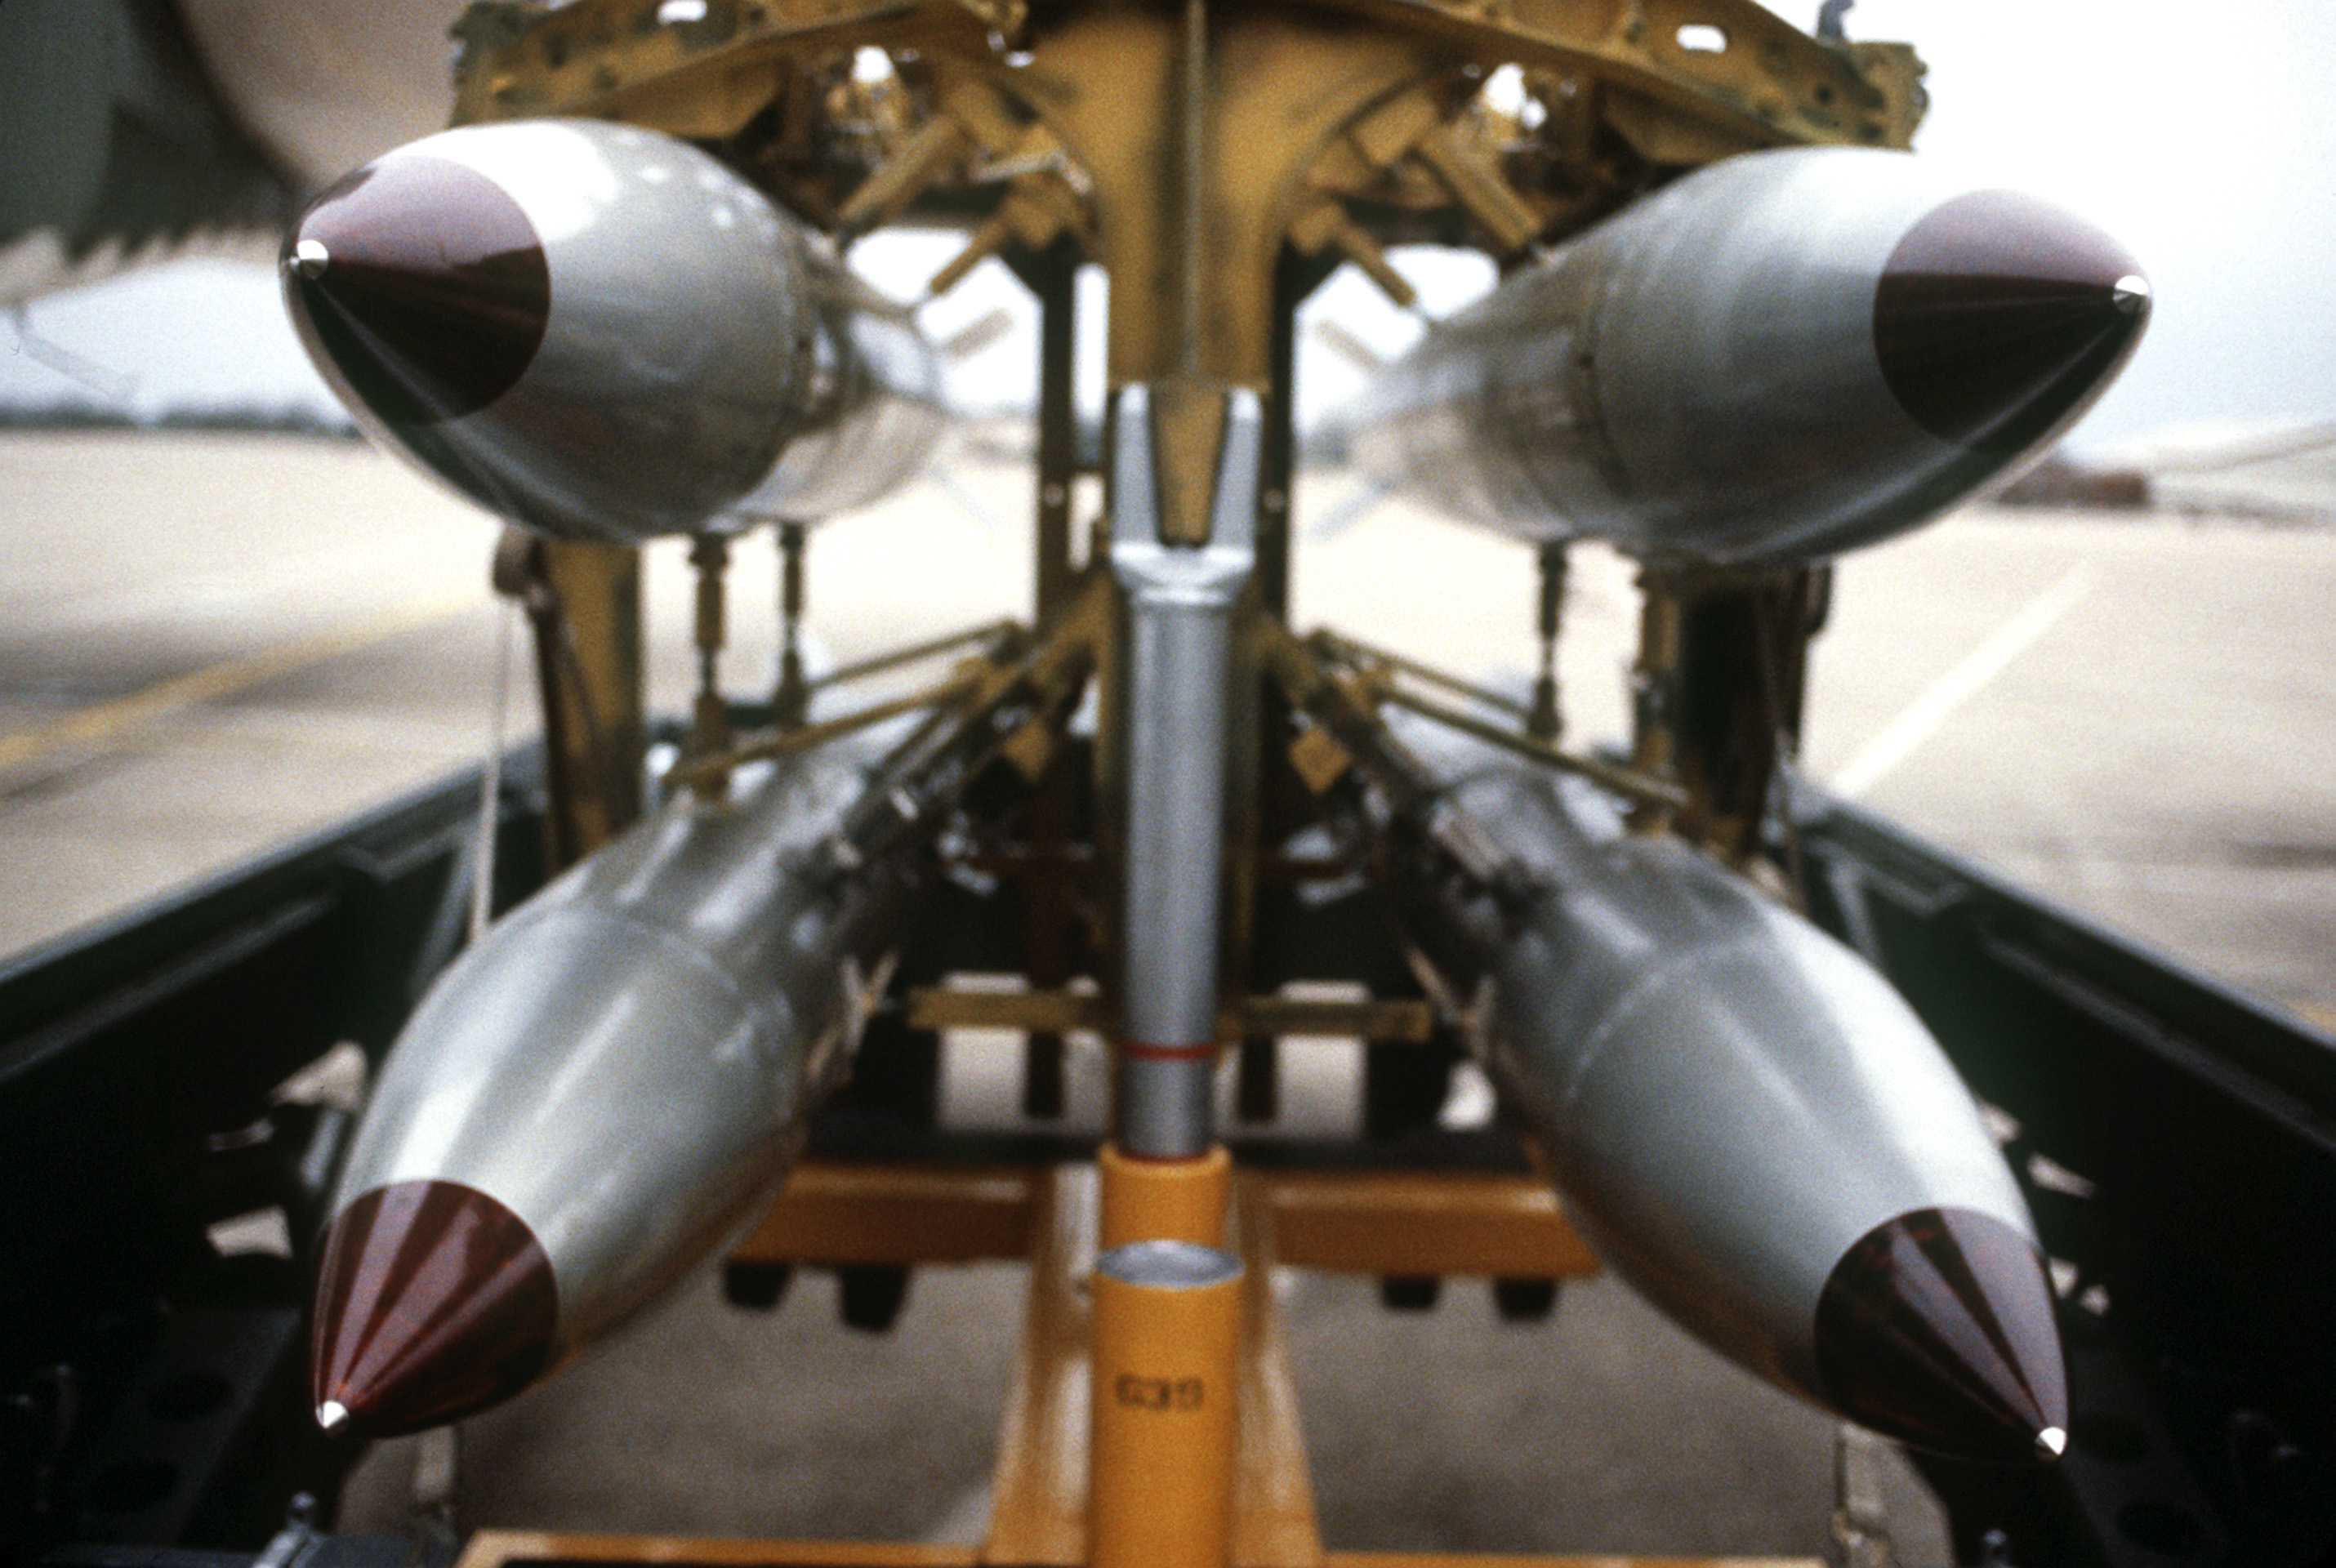
\includegraphics[width=\textwidth]{images/B-61_bomb_rack.jpg}
\end{block}
\end{column}
\end{columns}

\begin{columns}
\begin{column}{0.48\textwidth}
\tiny \textcolor{gray}{CC-BY-SA Stahlkocher}
\end{column}

\begin{column}{0.48\textwidth}
\tiny \textcolor{gray}{Public Domain, U.S. DoD}
\end{column}
\end{columns}
\end{frame}


\section{Disarmament}
\label{sec-2}
\begin{frame}[label=sec-2-1]{Present Arms Control}
\begin{columns}[t]

\begin{column}{0.48\textwidth}
\begin{block}{Non-Proliferation Treaty}
Entered into force in 1970

Defines \alert{Nuclear Weapon States} and \alert{Non-Nuclear Weapon States}

Prohibits development of nuclear weapons for latter.
\end{block}
\end{column}

\begin{column}{0.48\textwidth}

\vspace{0.1cm}

Partial Test Ban Treaty:\\
     Bans nuclear weapon testing in atmosphere, under water and on surface.\\[1.2em]

Several other smaller treaties exist, often only bilateral between Russia and the United States.
\end{column}
\end{columns}
\end{frame}

\begin{frame}[label=sec-2-2]{Future Regulation}
\begin{block}{Comprehensive Test Ban Treaty (CTBT)}
Banning all testing, including underground testing.\\
      International Monitoring System already in place \alert{and working}\\
      (e.g. North Korea).
\end{block}


\begin{block}{Fissile Material Cut-off treaty}
Ban production of weapon-usable fissile material.
\end{block}


\begin{block}{Disarmament Treaty}
Not yet discussed!

Nuclear Weapons Convention / Ban-Treaty / \ldots{}?
\end{block}
\end{frame}

\begin{frame}[label=sec-2-3]{}

\begin{center}
Independent of political solutions: \\[0.3em]
\Large
There are\\ many technical problems and challenges\\ without a solution.\\[1em]

\pause

Complicated task - Help from every community needed!
\end{center}
\end{frame}

\begin{frame}[label=sec-2-4]{Disarmament Verification}
\begin{varblock}[\textwidth]{}
\centering
Process of warhead dismantlement\\[0.7em]
 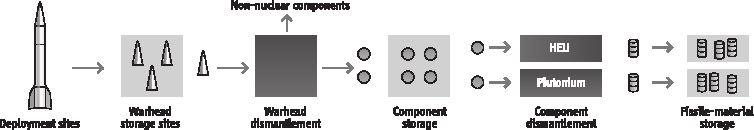
\includegraphics[width=\textwidth]{images/warhead_dismantlement}
\end{varblock}

\begin{tikzpicture}[remember picture, overlay]
\node [shift={(5.7cm, 0.8cm)},rotate = 90] at (current page.center) {\tiny \textcolor{gray}{CC-BY-SA - IPFM}};
\end{tikzpicture}

\begin{block}{Verification}
\begin{center}
Carried out to have high confidence in number / location\\ of dismantled warheads.

Should include participation of non-nuclear weapon states.
\end{center}
\end{block}
\end{frame}

\begin{frame}[label=sec-2-5]{Verification Goal}
\begin{center}
Is there a bomb in the box?
\end{center}

\begin{columns}
\begin{column}{0.18\textwidth}
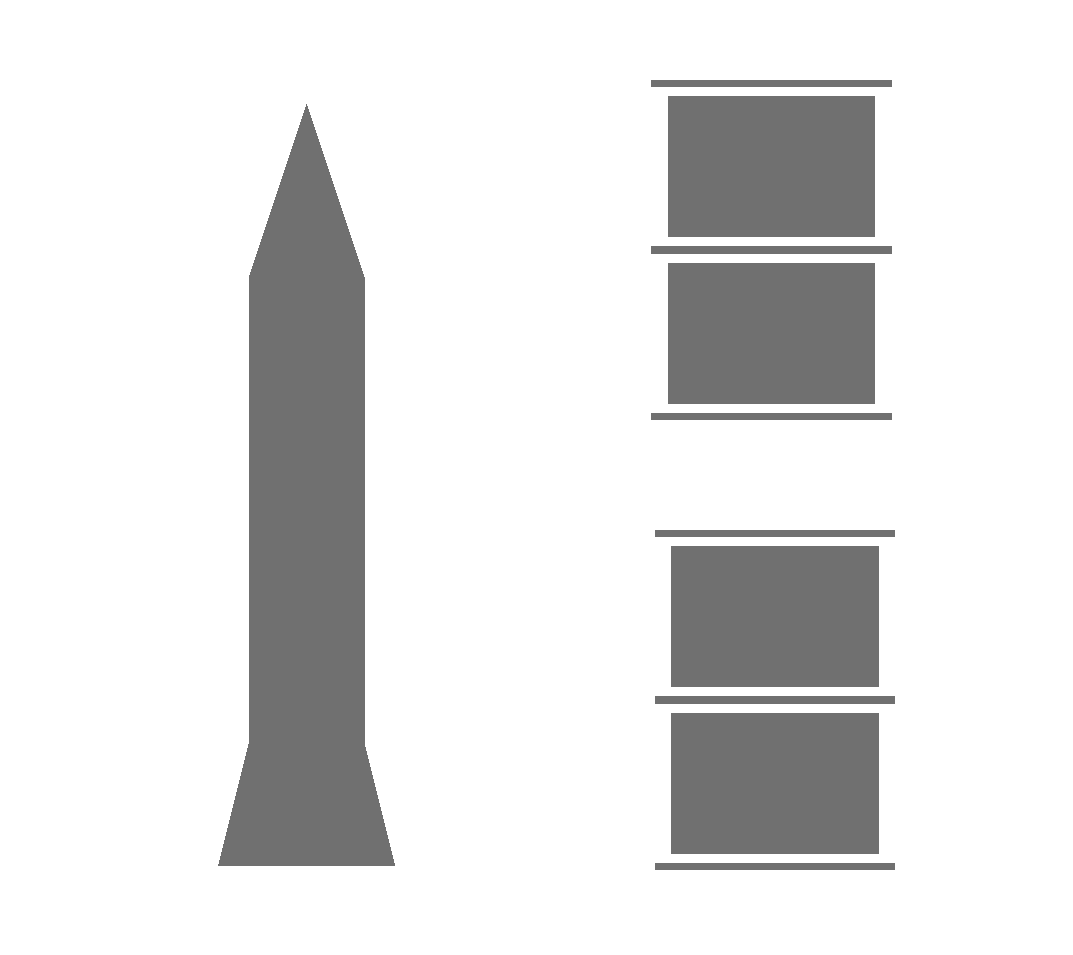
\includegraphics[width=\textwidth]{images/ib/box_visible}
\end{column}
\begin{column}{0.28\textwidth}
\small
Host Party (Host) owns weapon ready for dismantlement, or spoof.
\end{column}

\begin{column}{0.18\textwidth}

\includegraphics[width=\textwidth]{images/ib/box_transparent}
\end{column}
\begin{column}{0.28\textwidth}
\small
Inspecting Party (Inspector) needs to verify weapon / spoof without opening the box.
\end{column}
\end{columns}


\vfill
Two Approaches:
\begin{columns}

\begin{column}{0.48\textwidth}
\begin{block}{Template Approach}
\small
Items are compared to "Golden Sample", which identity is proved by other means.
\end{block}
\end{column}

\begin{column}{0.48\textwidth}
\begin{block}{Attribute Approach}
\small
Items are checked for particular attributes (e.g. presence/mass of fissile material).
\end{block}
\end{column}
\end{columns}
\end{frame}

\begin{frame}[label=sec-2-6]{Further Complication}

Adherance to existing regulation in the Non-Proliferation Treaty required:

\begin{quote} %% Art. I
\small
Article I\\
Each nuclear-weapon State Party to the Treaty undertakes [\ldots{}] not in any way to assist, encourage, or induce any non-nuclear-weapon State to manufacture or otherwise acquire nuclear weapons or other nuclear explosive devices, or control over such weapons or explosive devices.
\end{quote}


In addition, states claim information sensitivity / classification because of national security interests.
\end{frame}



\section{Free Software}
\label{sec-3}
\begin{frame}[label=sec-3-1]{}
\begin{center}
Hack 1: Free Software
\end{center}
\end{frame}

\begin{frame}[label=sec-3-2]{}

\begin{center}
\Large

Software is used\\
to develop new measurement technologies\\
and during implementation of disarmament verification\\[1.5em]

\color{gray!50}{\small (also needs hardware and institutional arrangements...)}
\end{center}
\end{frame}


\begin{frame}[label=sec-3-3]{Neutron Multiplicity Measurements}

\begin{tikzpicture}[remember picture,overlay]
    {{\uncover<1->{\node [shift={(-1.7cm,0.8cm)}, line width=1mm, draw=black, inner sep=0pt] at (current page.center) {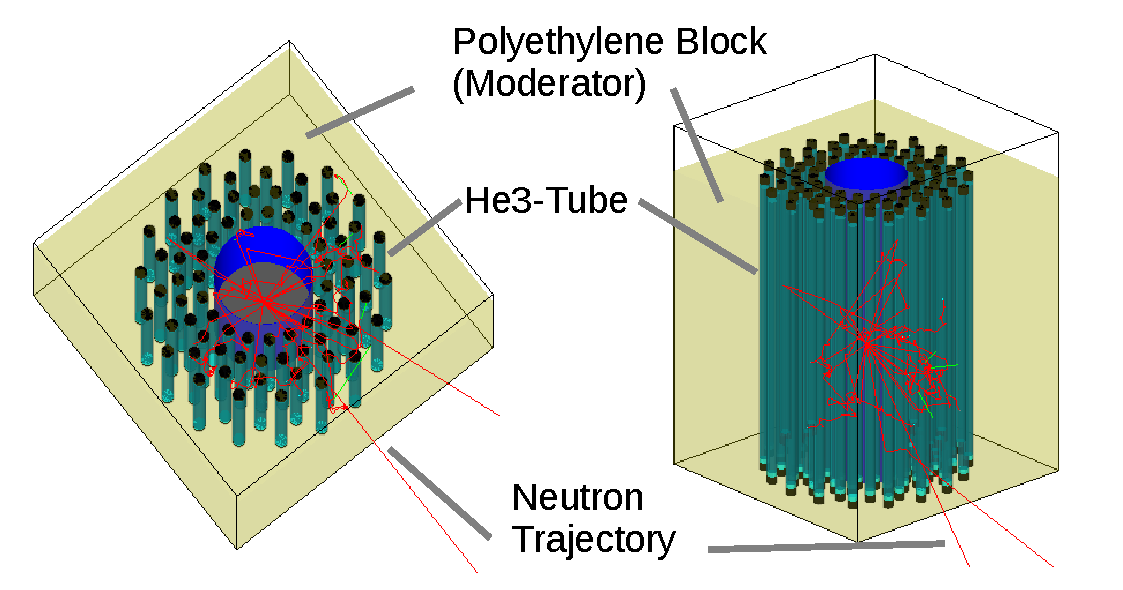
\includegraphics[width=8cm]{images/nms/detector}};}}};
    {{\uncover<2->{\node [shift={(0cm,-1.9cm)}, line width=1mm, draw=black,inner sep=0pt] at (current page.center) {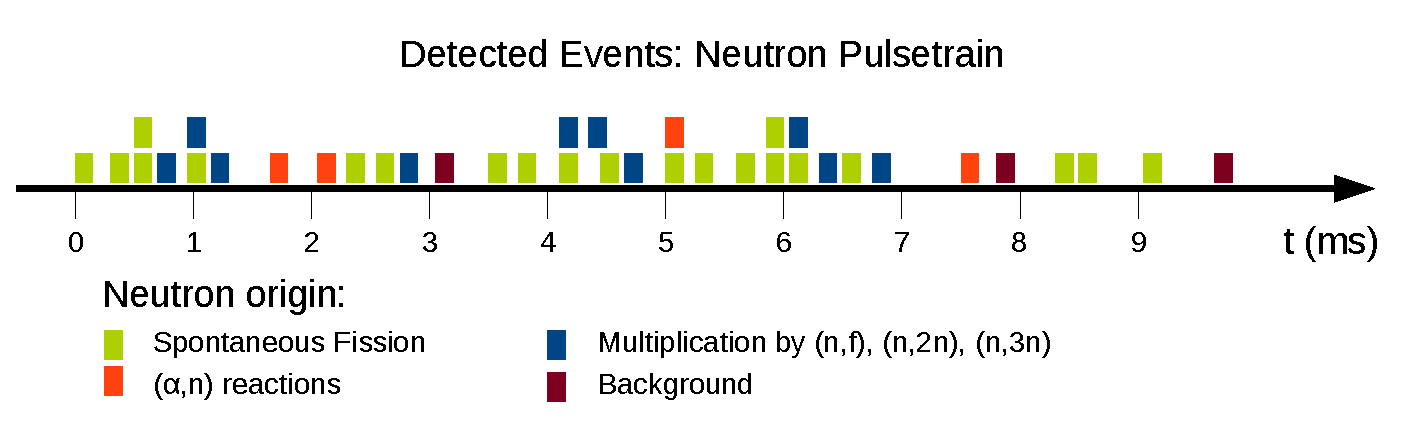
\includegraphics[width=11cm]{images/nms/pulsetrain_title}};}}};
    {{\uncover<3->{\node [shift={(4cm,0.5cm)}, line width=1mm, draw=black,inner sep=0pt] at (current page.center) {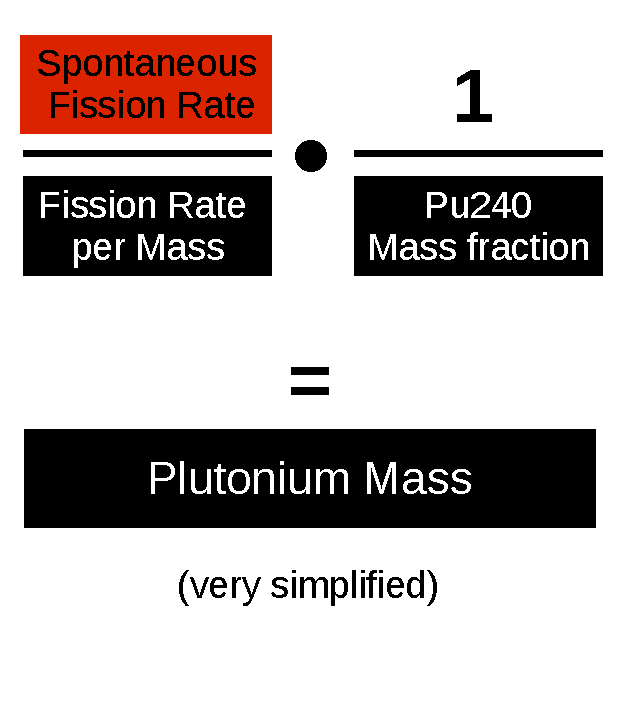
\includegraphics[width=4cm]{images/nms/math_2}};}}};
\end{tikzpicture}
\end{frame}


\begin{frame}[label=sec-3-4]{Problem}

\begin{alertblock}<1->{Currently used software often suffers from}
Difficulties for software verification (no source code access)\\[0.35em]
Limited application and development (“expert communties”)\\[0.35em]
Limited access (export controls)\\[0.35em]
(High) financial requirements\\[0.35em]
\end{alertblock}

\begin{block}<2->{How to establish trust\ldots{}}
if software is used as tools for decision making?\\[0.5em]
if states rely on results of software?
\end{block}
\end{frame}



\begin{frame}[label=sec-3-5]{}

\begin{center}\Large
Free Software criteria for software in Nuclear Arms Control!
\end{center}

\begin{exampleblock}{Three Criteria derived from Free Software / Open Source}
(1) No restrictions for access to program.

(2) Distribution of program must include full source code.

(3) Modifications of the program are allowed to anybody.
\end{exampleblock}

\hfill
\hfill


\begin{columns}
\begin{column}{0.45\textwidth}

\begin{varblock}[\textwidth]{}
\begin{minipage}[c]{0.5\linewidth}

\includegraphics[width=0.9\textwidth]{images/fsf-only}
\end{minipage}\hfill
\begin{minipage}[c]{0.5\linewidth}
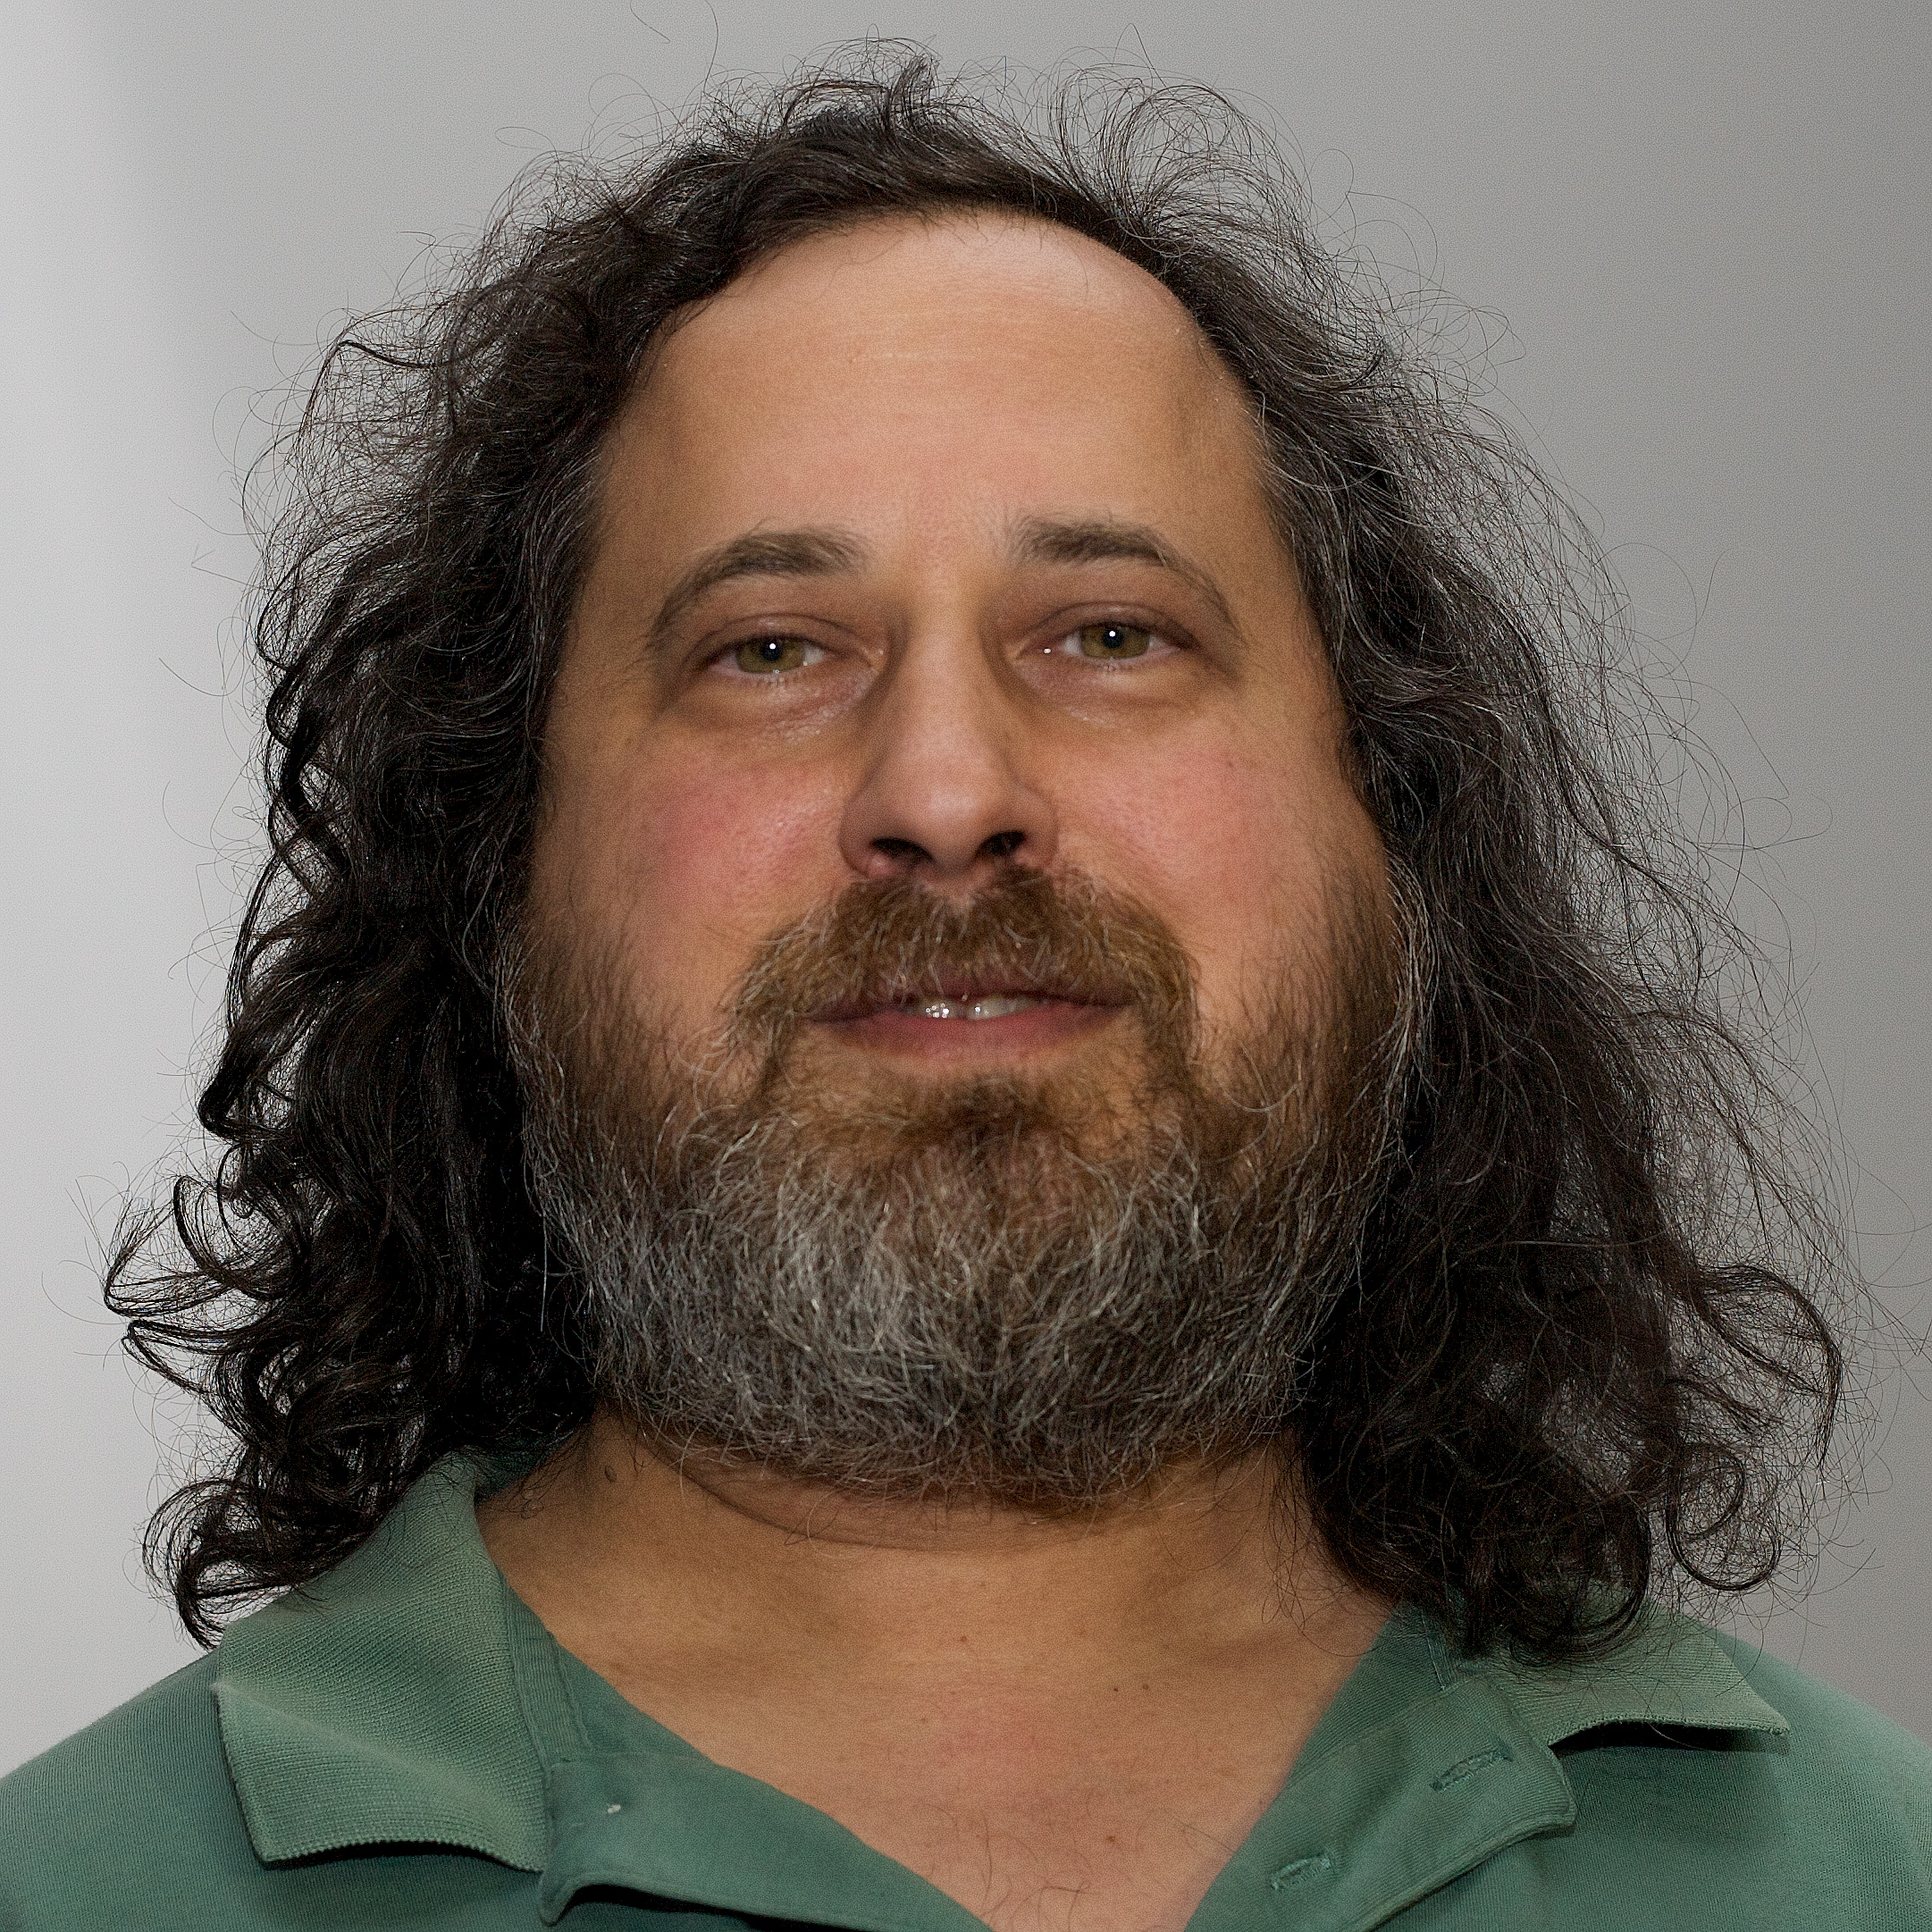
\includegraphics[width=0.9\textwidth]{images/NicoBZH_-_Richard_Stallman_(by-sa)_(5).jpg}
\end{minipage}
\end{varblock}
\vspace{-0.6cm}
\begin{minipage}[c]{0.5\linewidth}
    \tiny \textcolor{gray}{Public Domain}
\end{minipage}\hfill
\begin{minipage}[c]{0.5\linewidth}
\tiny \textcolor{gray}{CC-BY-SA NicoBZH}
\end{minipage}
\vspace{-0.2cm}
\end{column}

\begin{column}{0.45\textwidth}
\begin{varblock}[\textwidth]{}
\begin{minipage}[c]{0.5\linewidth}

\includegraphics[width=0.75\textwidth]{images/Opensource}
\end{minipage}\hfill
\begin{minipage}[c]{0.5\linewidth}
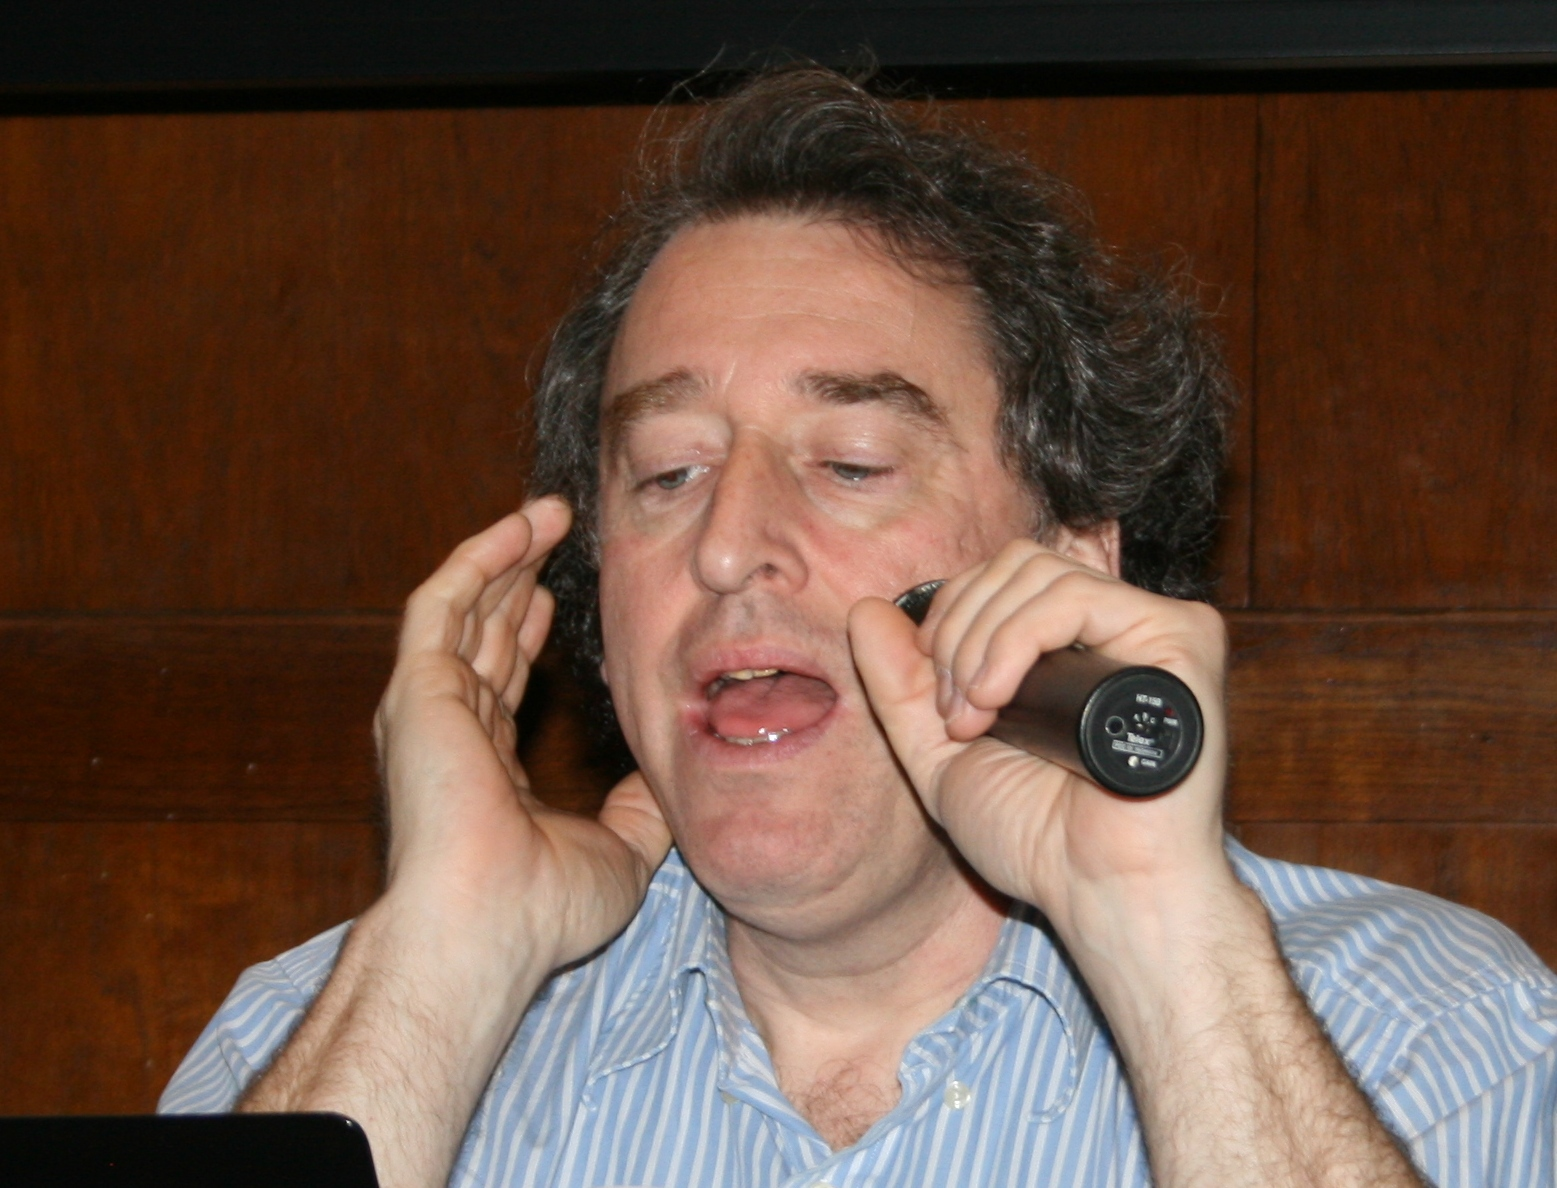
\includegraphics[width=0.9\textwidth]{images/Bruce_perens_13jan09_tacd_MAR_1557x1188.JPG}
\end{minipage}
\end{varblock}
\vspace{-0.4cm}
\begin{minipage}[c]{0.5\linewidth}
\tiny \textcolor{gray}{CC-BY Open Source\newline Initiative}
\end{minipage}\hfill
\begin{minipage}[c]{0.5\linewidth}
\tiny \textcolor{gray}{CC-BY-SA Manon\newline Anne Ress}
\end{minipage}
\end{column}
\end{columns}

\begin{tikzpicture}[overlay,line width=0.1cm]
        \path[->,white] (2.3,3.2) edge (3.3,4);
        \path[->,white] (8.3,3.2) edge (7.3,4.);
        \path[<->,white] (5.1,1.8) edge (5.7,1.8);
\end{tikzpicture}
\end{frame}


\begin{frame}[label=sec-3-6]{Prevent Backdoors/Cheating}
Kerckhoffs' principle (cryptography)

\begin{quote} %% Kerckhoffs principle
Il faut qu’il n’exige pas le secret, et qu’il puisse sans inconvénient tomber entre les mains de l’ennemi;\\[0.3em]

\footnotesize (It must not require secrecy, and can without concerns fall into enemy hands.)

\vskip1mm \hspace*\fill{\tiny--- Auguste Kerckhoffs, La cryptographie militaire 1883, IX, 5-38, 161-191}
\end{quote}



\vfill

\begin{block}{"Verification of the Verification"}
\begin{center}
Inspected \& Inspecting Party can review functionality\\ of Open Source Software
\end{center}
\end{block}
\end{frame}

\begin{frame}[label=sec-3-7]{Increase Participation}
\begin{block}{Three groups}
\begin{tabular}{ll}
\alert{Verification Experts} & Nuclear Technical community\\
\alert{Other Experts} & Academia, technical communities, \\
& not related to Arms Control \\
\alert{Society} & Public, laypersons \\
\end{tabular}
\end{block}

\begin{block}{Open Source}
\begin{itemize}
\item \textcolor{black}{enables connection between communities}
\item \textcolor{black}{verification supported beyond arms control community}
\item \textcolor{black}{to involve of society, Crowd-Sourcing / Societal Verification}
\end{itemize}
\end{block}
\end{frame}


\begin{frame}[label=sec-3-8]{}

\begin{center}

Work on this issue is part of my PhD project.\\[1em]

www.nuclearfreesoftware.org \\[3em]
\end{center}


\footnotesize

M. Kütt, A. Glaser and M. Englert. "Open Source meets Nuclear Arms Control", In: Proceedings of 55th Annual INMM Meeting, Atlanta, GA, 21-24 July 2014.\\[0.3em]

M. Kütt and M. Englert. "Increased transparency in simulations of measurements for nuclear disarmament verification", In: F. Sevini (Ed.). 35th ESARDA Symposium proceedings, Bruges, 27-30 May 2013.


\pause

\normalsize

\vspace{0.8cm}

\begin{center}
\emph{Can you imagine to help?}
\end{center}
\end{frame}

\section{Information Barrier}
\label{sec-4}
\begin{frame}[label=sec-4-1]{}

\begin{center}
Hack 2: Information Barrier
\end{center}
\end{frame}


\begin{frame}[label=sec-4-2]{Information Barrier}
\begin{center}
Measurement of classified/sensitive physical quantity (e.g. attribute)\\[1.5em]
\end{center}

\begin{columns}
\begin{column}{0.48\textwidth}
\begin{varblock}[\textwidth]{}
    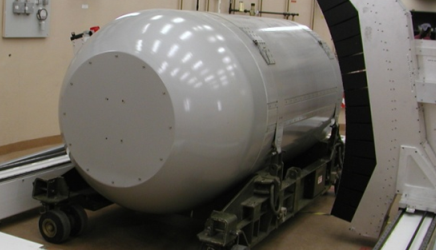
\includegraphics[width=\textwidth]{images/2013-09-30_na22_3_topline.png}
\end{varblock}
\vspace{-0.3cm}
    \tiny \textcolor{gray}{Public Domain - U.S. DoE NNSA}
\end{column}



\begin{column}{0.48\textwidth}
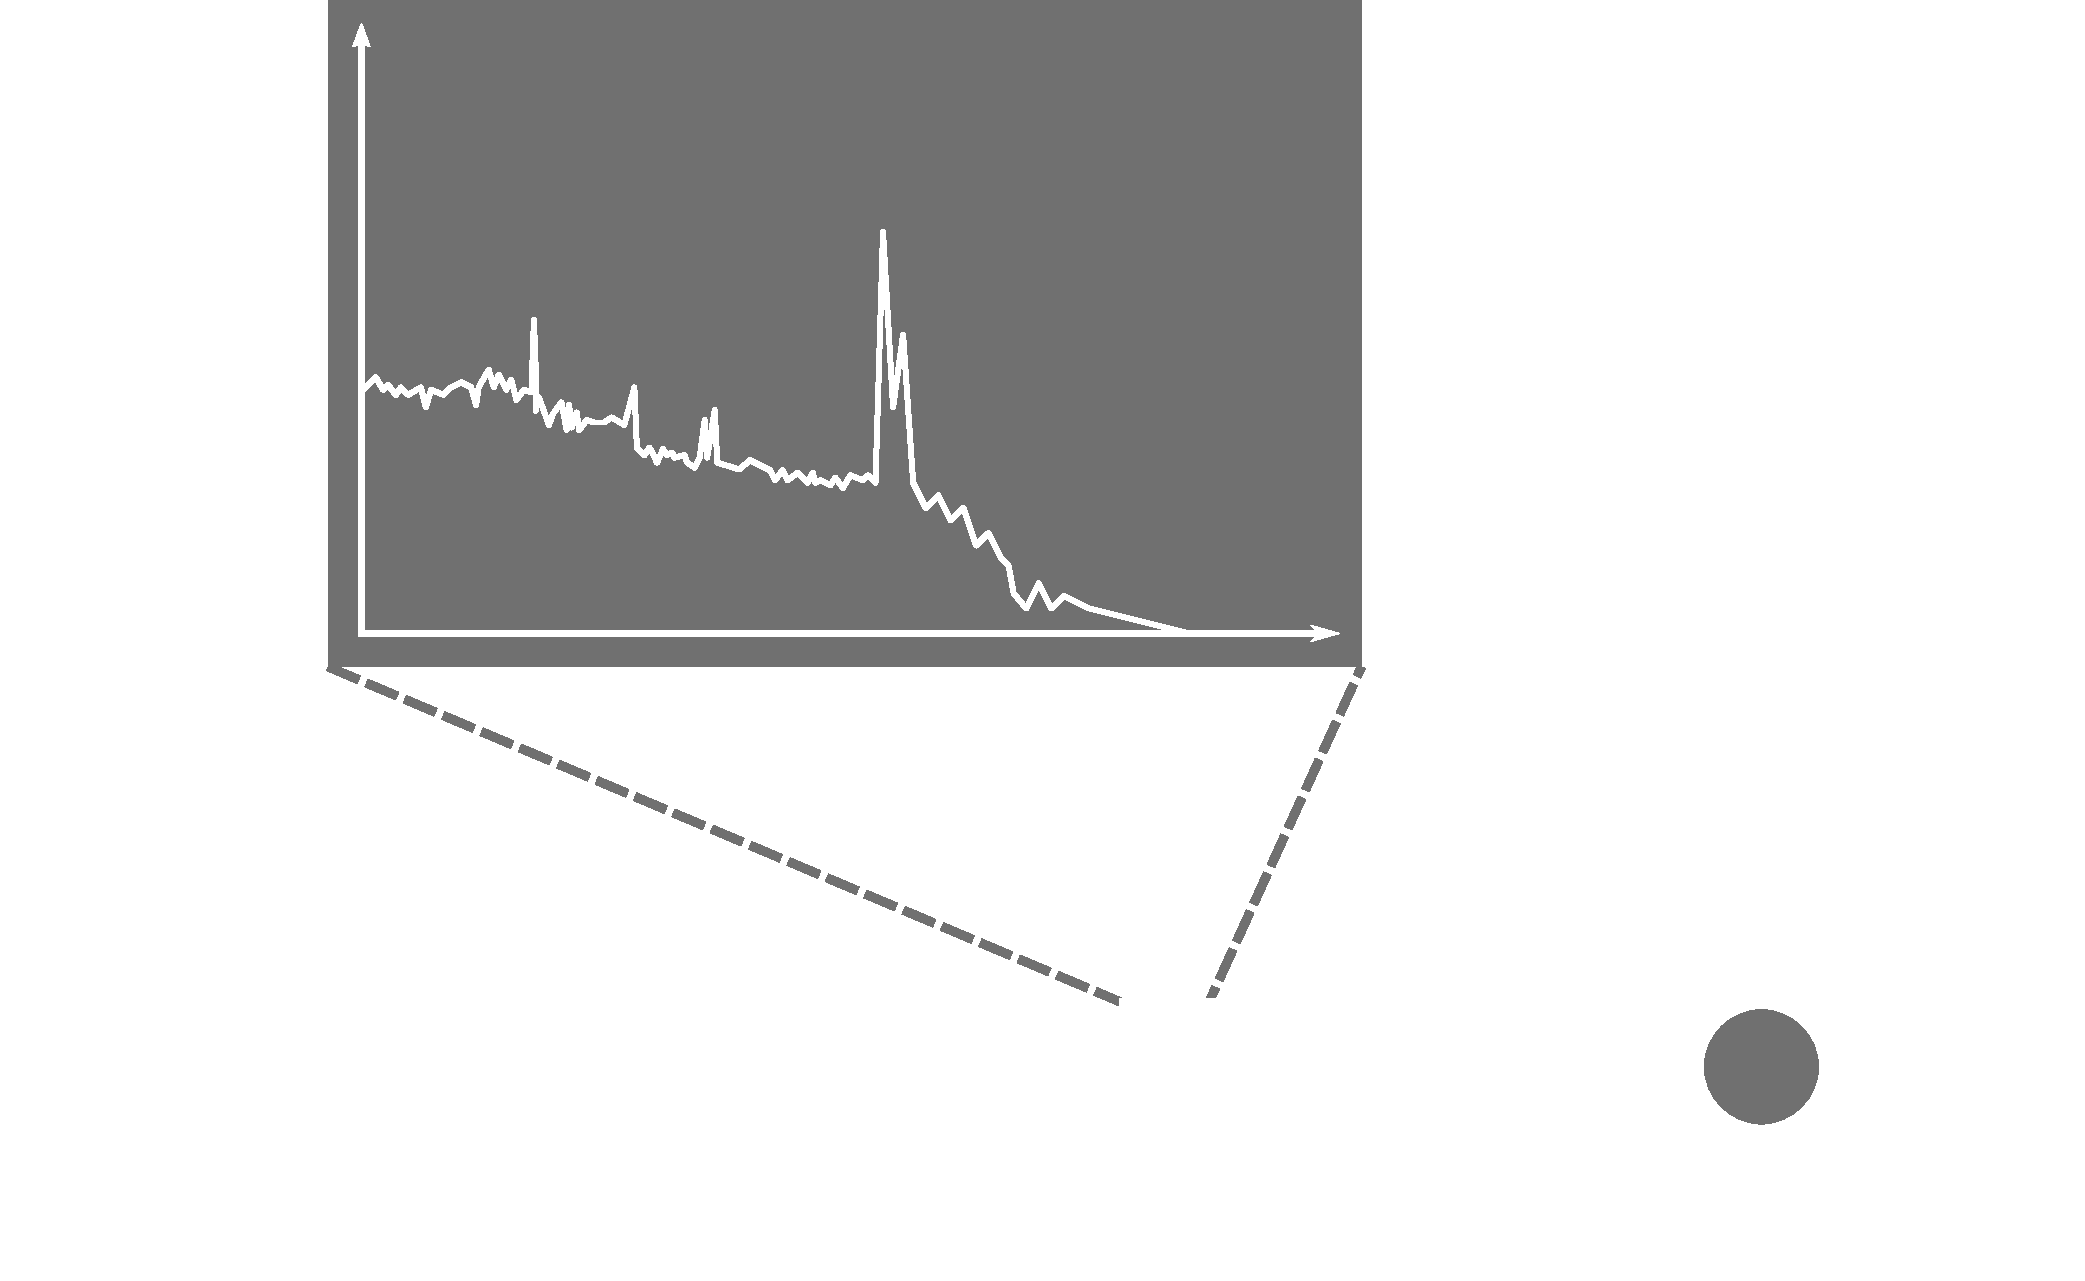
\includegraphics[width=\textwidth]{images/ib/ib_classified}
\end{column}
\end{columns}
\end{frame}

\begin{frame}[label=sec-4-3]{Information Barrier}
\begin{center}
Classified information transformed into unclassified information:
\end{center}

\begin{columns}
\begin{column}{0.48\textwidth}
Information barrier shows simple information to inspector\\[1.5em]


\includegraphics[width=\textwidth]{images/ib/ib_good}
\end{column}

\begin{column}{0.48\textwidth}
But should be able to detect cheating\\[1.5em]

\includegraphics[width=\textwidth]{images/ib/ib_bad}
\end{column}
\end{columns}


\begin{center}
Typically based on jointly developed hardware/software.
\end{center}
\end{frame}

\begin{frame}[label=sec-4-4]{Development Examples}
\begin{block}{Trilateral Initiative (90s)}
Russia, USA and International Atomic Energy Agency.

Research mechnologies / methods to verify fissile material coming from nuclear weapons.
\end{block}

\begin{block}{UK-Norway-Initiative (2010-2015)}
Exercise for verified warhead dismantlement.

Research: Social issues (inspector / host), development of information barrier.
\end{block}
\end{frame}


\begin{frame}[label=sec-4-5]{Challenges}
\begin{columns}
\begin{column}{0.48\textwidth}
\tcbset{redheight/.style={tcbeamer,valign=center,center upper,notitle,colframe=red!85,equal height group=reds,colback=red!85}}
\begin{tcolorbox}[redheight]
{\bf Hardware Verification} \\ (e.g. Hardware Trojans?)
\end{tcolorbox}
\begin{tcolorbox}[redheight]
{\bf Software Verification} \\ (Backdoor / Cheating)
\end{tcolorbox}
\visible<3->{
\begin{tcolorbox}[redheight]
{\bf Host Provided Hardware} \\ "Warhead" Certified
\end{tcolorbox}
\begin{tcolorbox}[redheight]
{\bf Quality / Validity} \\ of Measurements
\end{tcolorbox}
}
\end{column}


\begin{column}{0.48\textwidth}

\visible<2->{
\begin{center}
Could you trust this system?
\end{center}

\begin{varblock}[\textwidth]{}
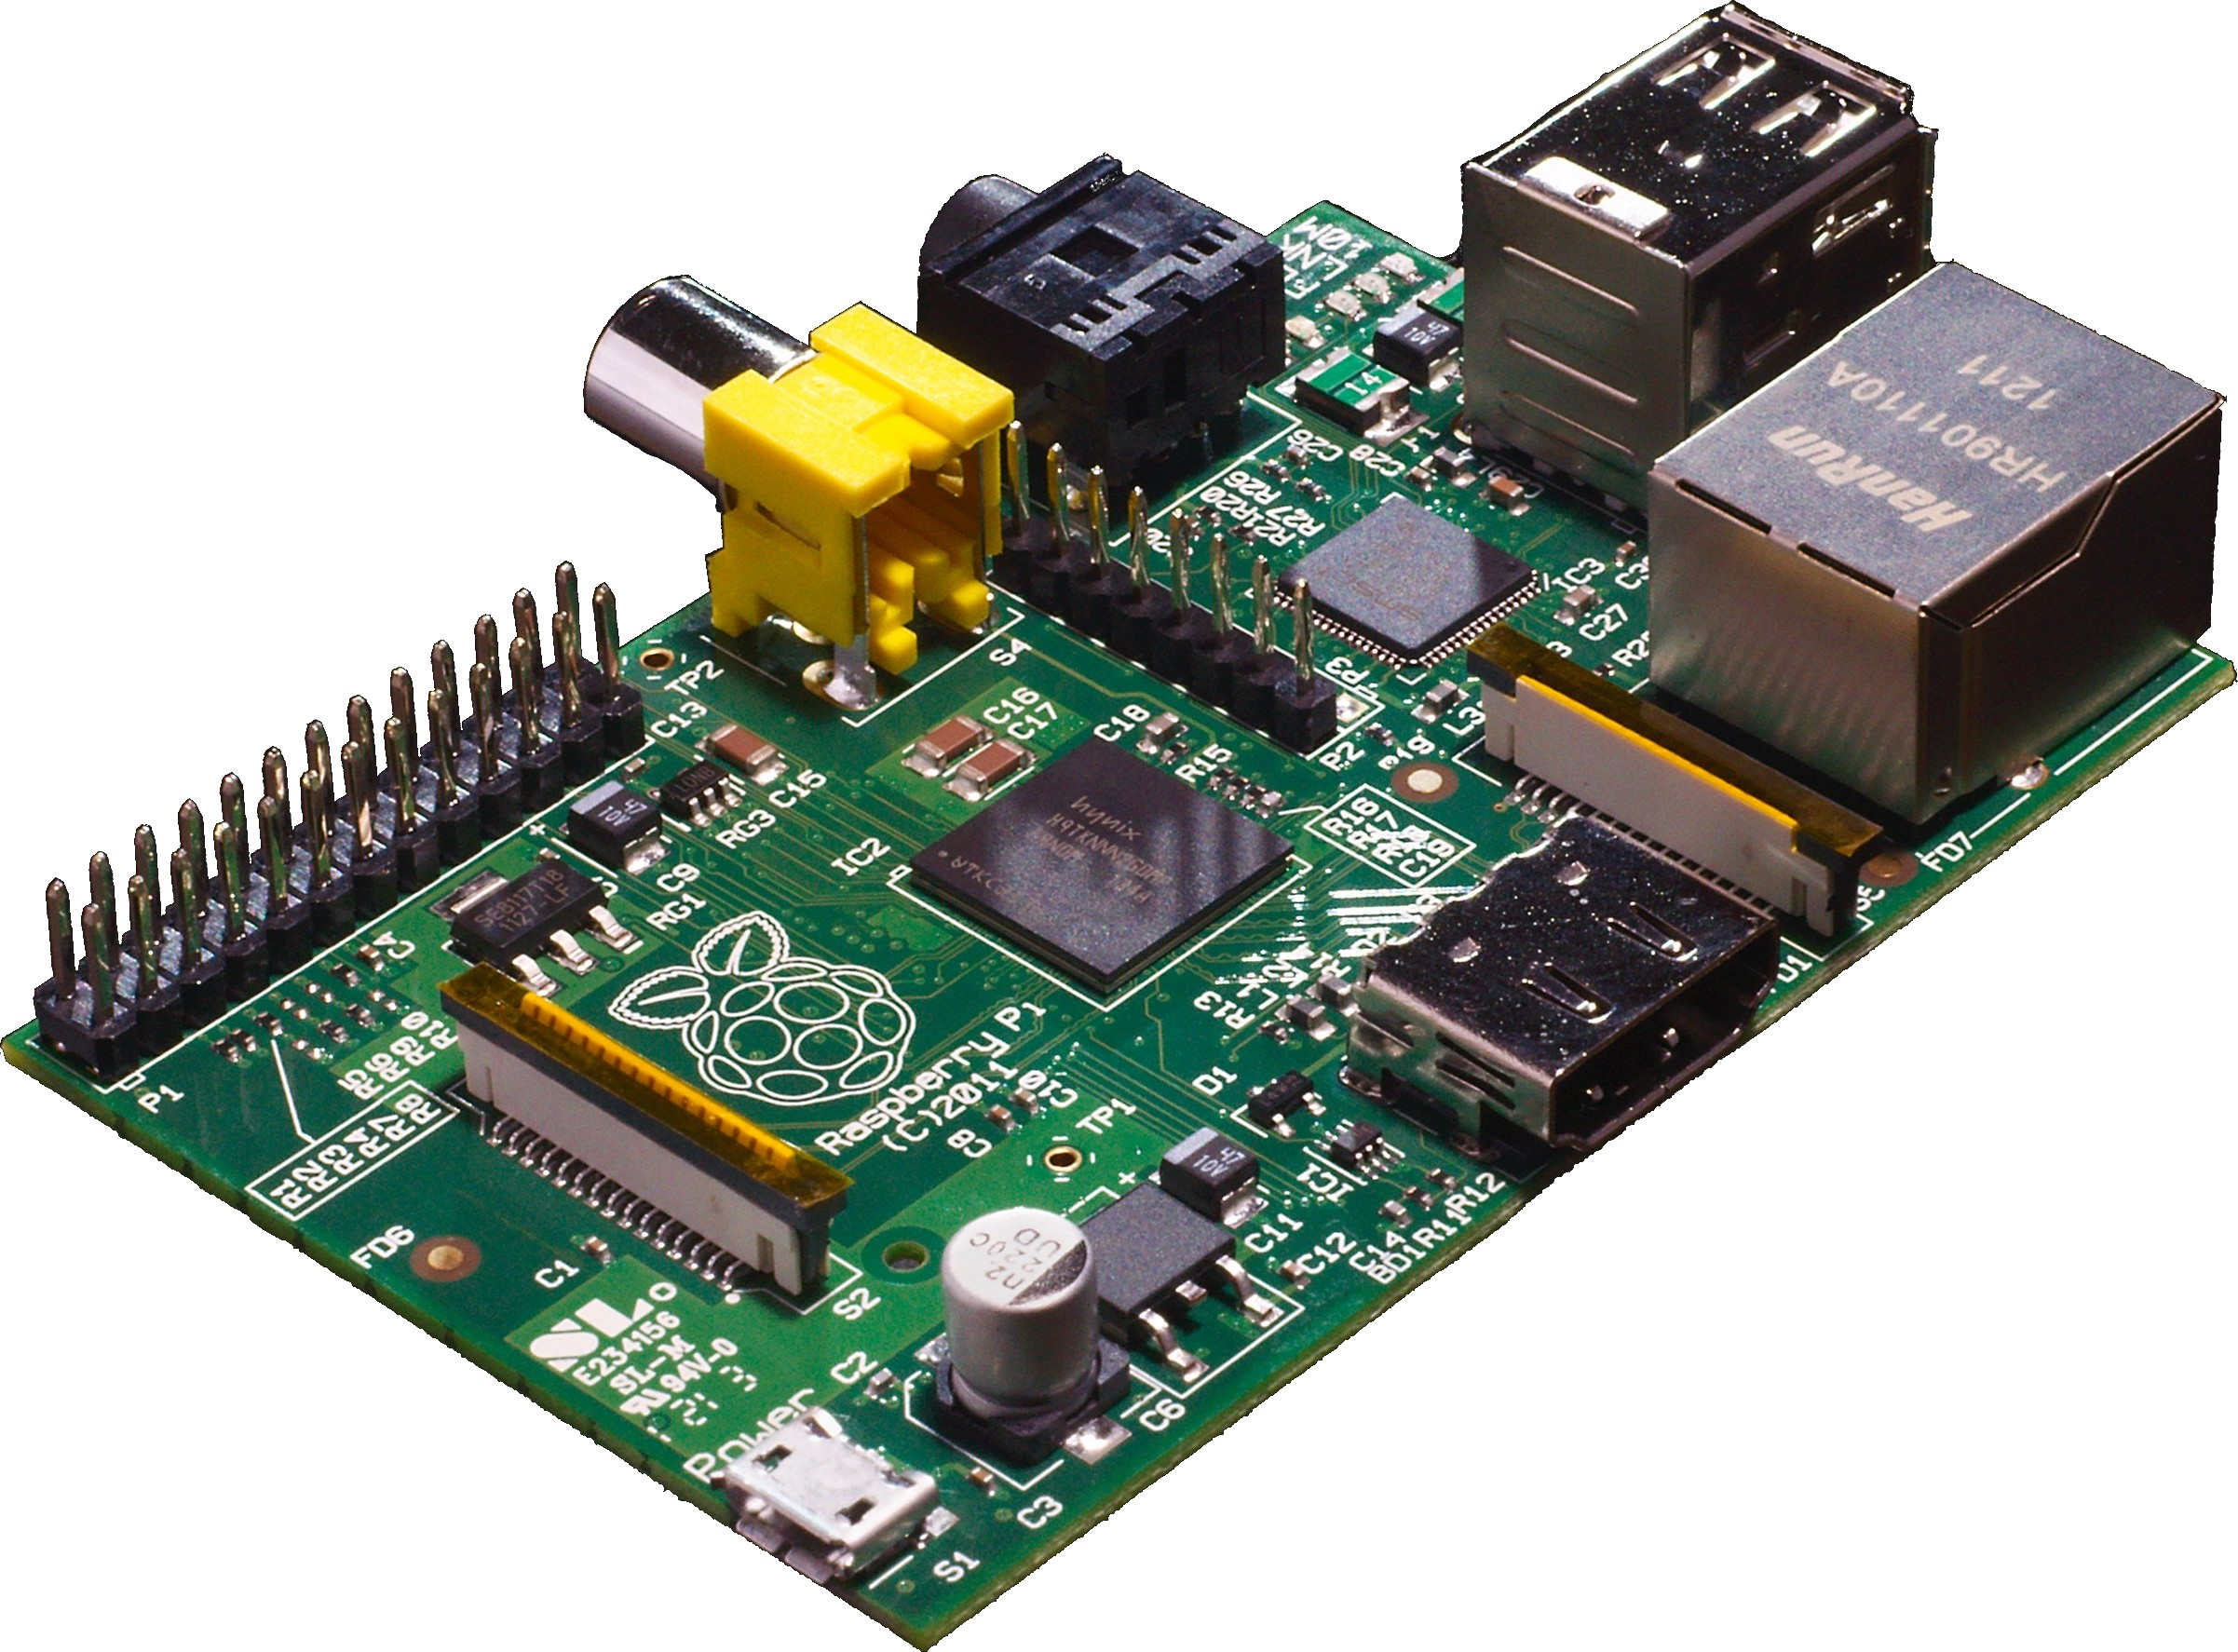
\includegraphics[width=\textwidth]{images/Raspberry_Pi_Photo.jpg}\\
\end{varblock}
\vspace{-0.3cm}
\tiny \textcolor{gray}{CC-BY-SA cowjuice}
}
\end{column}
\end{columns}
\end{frame}


\begin{frame}[label=sec-4-6]{Current Research}
\footnotesize

J. Fuller. "The functional Requirements and Design Basis for Information Barriers", Report PNNL-13285, Pacific Northwestern National Laboratory, 1999.\\[0.3em]

K. Allen et al. "UK-Norway Initiative (UKNI) approach for the development of a Gamma Ray Attribute Measurement System with an integrated Information Barrier", In: F. Sevini (Ed.), proceedings of 35th ESARDA Symposium proceedings, Bruges, 27-30 May 2013.\\[0.3em]

M. Göttsche and G. Kirchner. "Measurement Techniques for Warhead Authentication with Attributes: Advantages and Limitations," \emph{Science \& Global Security}, 22, no. 2, 2014.\\[0.3em]

(more \ldots{})


\pause

\vspace{1cm}

\begin{center}
\emph{Can you imagine to help?}
\end{center}
\end{frame}

\section{Zero-Knowledge}
\label{sec-5}
\begin{frame}[label=sec-5-1]{}
\begin{center}
Hack 3: Zero-Knowledge Protocol
\end{center}
\end{frame}
\begin{frame}[label=sec-5-2]{Basics}
\begin{block}{Cryptographic protocol}
\begin{itemize}
\item Proof a particular fact
\item Sound \& Complete
\item without revealing more knowledge
\end{itemize}

Required: \alert{Interaction} between parties
\end{block}
\end{frame}

\begin{frame}[label=sec-5-3]{Distinguishing Drinks}
\begin{center}
Can Bob distinguish two drinks? \\
\footnotesize Drinks look equal \\
(e.g. Coca Cola / Fritz Cola, French Wine / Californian Wine)
\end{center}

\begin{columns}[t]

\begin{column}{0.3\textwidth}
\footnotesize 
Bob tastes each drink and places them in Alice's right and left hand.\\[1cm]


\includegraphics[width=\textwidth]{images/zkp/step1.pdf}


\pause
\end{column}

\begin{column}{0.3\textwidth}
\footnotesize
Alice chooses to switch or not switch the cups (secretly).\\[1.3cm]


\includegraphics[width=\textwidth]{images/zkp/step2.pdf}

\pause
\end{column}

\begin{column}{0.3\textwidth}
\footnotesize
Bob tastes again and tells Alice if she switched.\\[1cm]

\normalsize
Repeating the game: More confidence in Bob's capabilities.
\end{column}
\end{columns}
\end{frame}

\begin{frame}[label=sec-5-4]{Nuclear Disarmament}
\begin{center}
Could be used for the Template approach.
\end{center}

\vspace{-0.7cm}

\begin{columns}
\begin{column}{0.48\textwidth}

\begin{center}
    Template

    
\includegraphics[width=0.6\textwidth]{images/zkp/template.pdf}
\end{center}
\end{column}

\begin{column}{0.48\textwidth}

\begin{center}
    Item

    
\includegraphics[width=0.6\textwidth]{images/zkp/item.pdf}
\end{center}
\end{column}
\end{columns}

\begin{block}{Idea (Glaser et al. 2014)}
Proof that templates are equal without revealing anything else\\[0.5em]

\begin{itemize}
\item measurement: neutron radiograph
\item preload detector with negative image
\item preload to match predefined result
\item inspector chooses placement of detector on template and item
\end{itemize}
\end{block}
\end{frame}




\begin{frame}[label=sec-5-5]{More practical\ldots{}}
\begin{columns}
\begin{column}{0.48\textwidth}

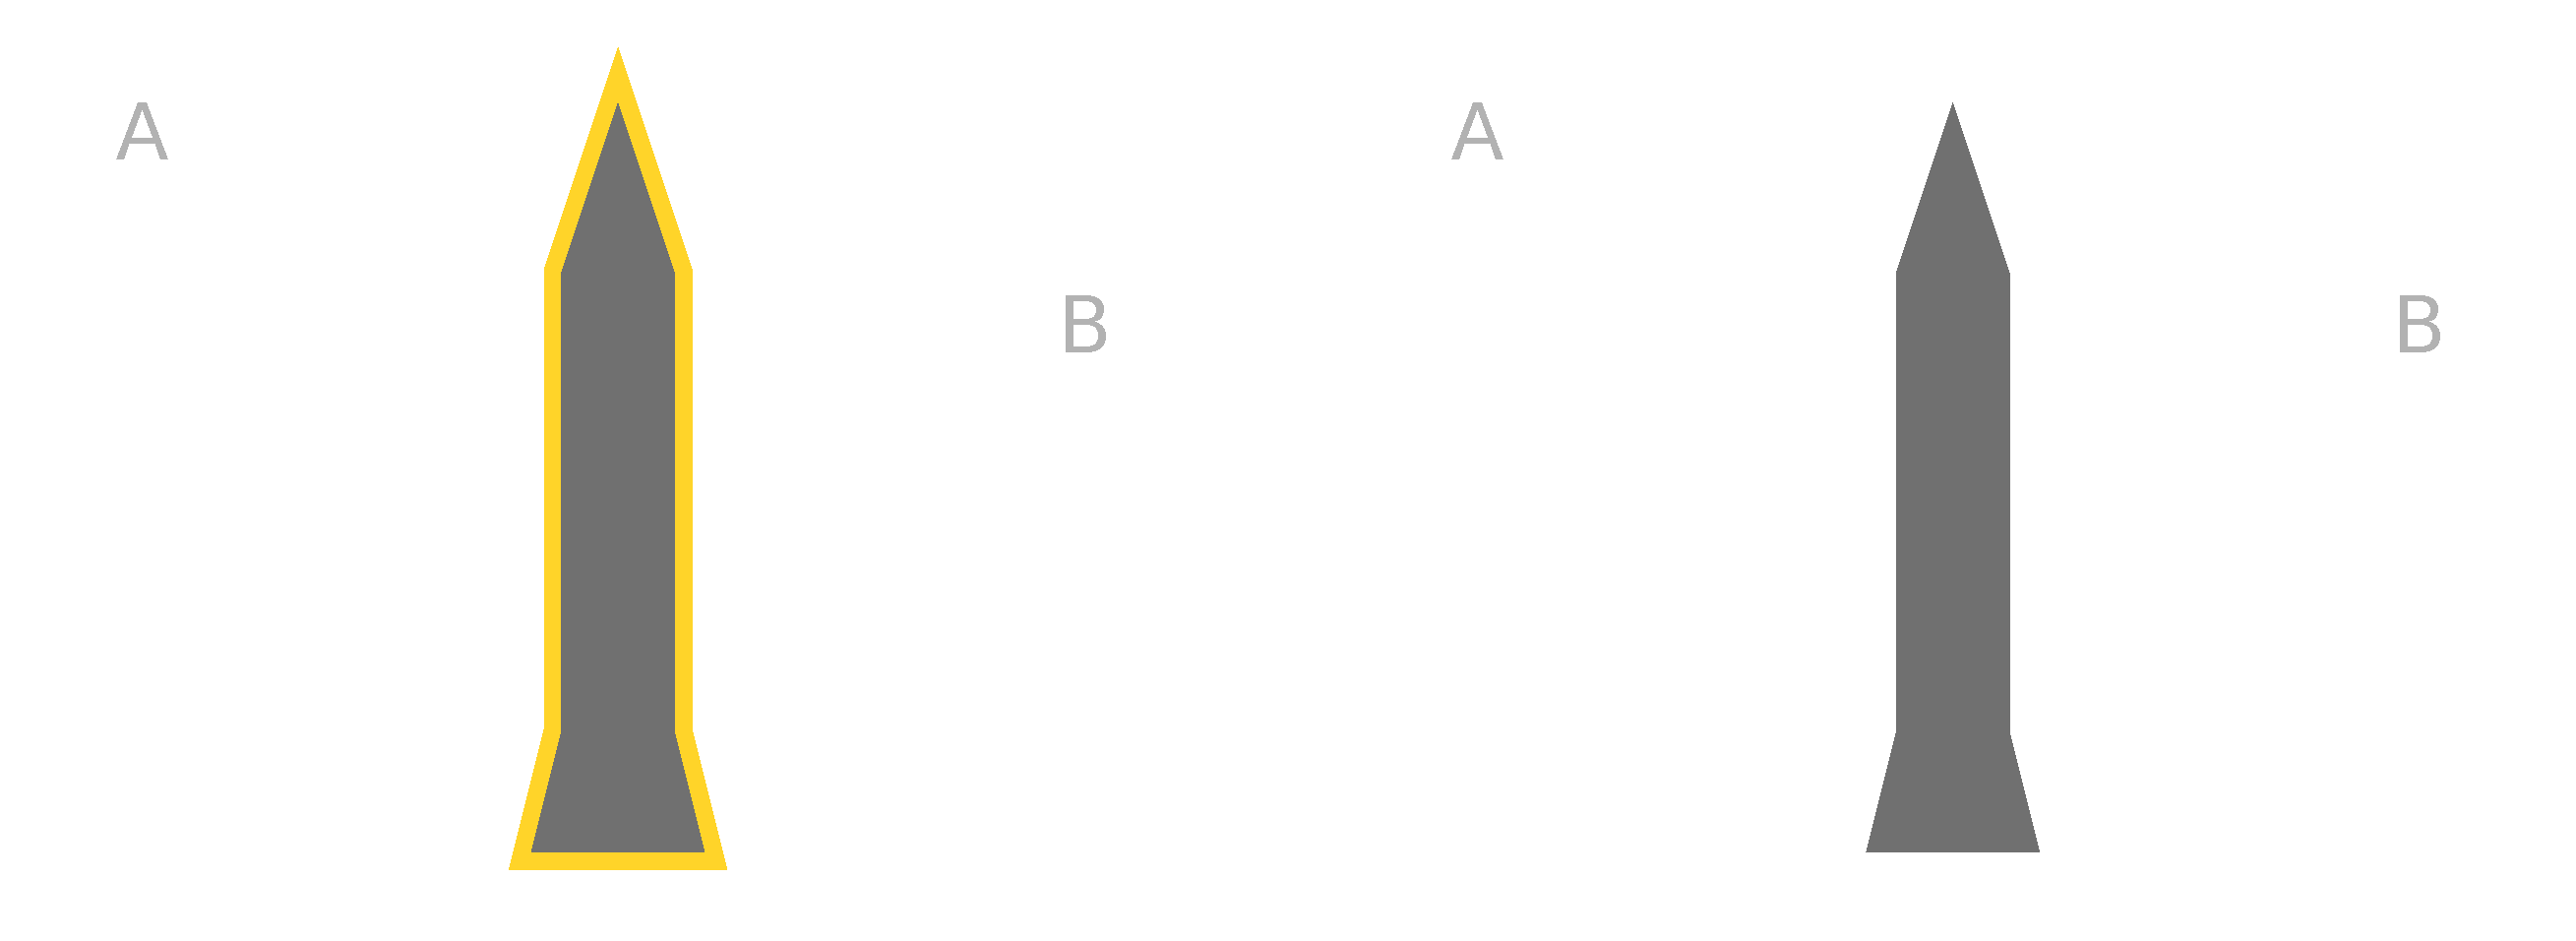
\includegraphics[width=\textwidth]{images/zkp/measurement_step1.pdf}
\vspace{1cm}

\pause

\begin{columns}
\begin{column}{0.48\textwidth}
\footnotesize Host preloads detectors with "negative image". \normalsize
\end{column}

\begin{column}{0.48\textwidth}

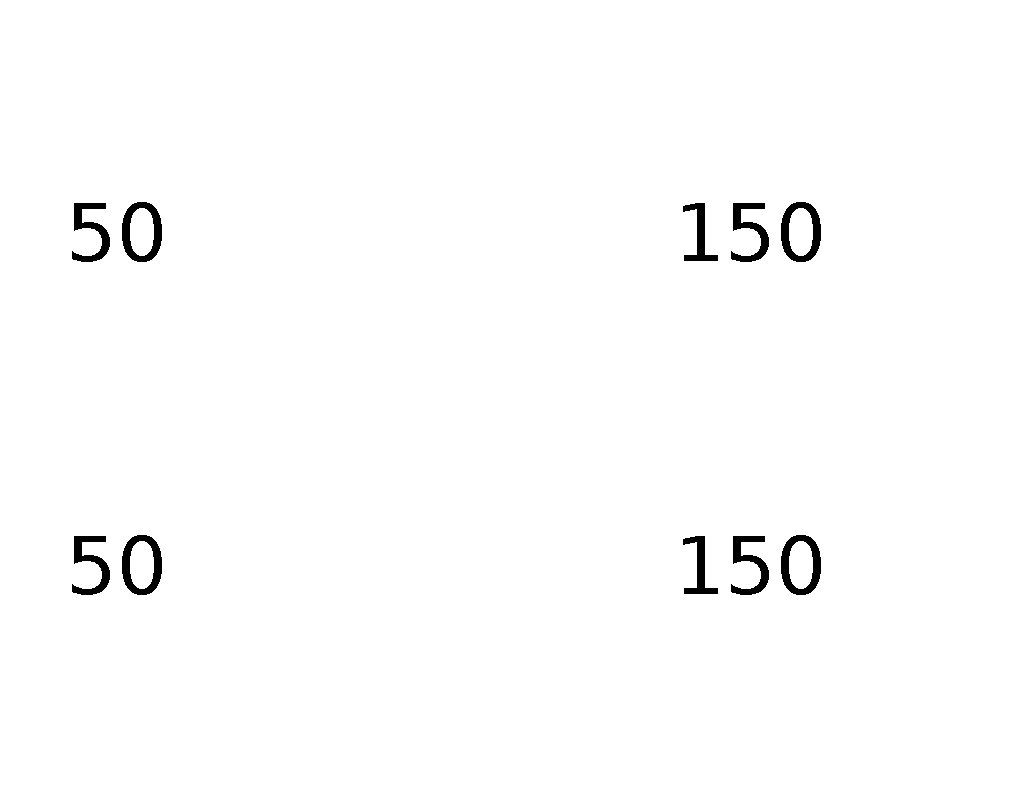
\includegraphics[width=\textwidth]{images/zkp/measurement_detectors_host.pdf}

\pause
\end{column}
\end{columns}
\end{column}

\begin{column}{0.48\textwidth}


\includegraphics[width=\textwidth]{images/zkp/measurement_step2.pdf}
\vspace{1cm}

\begin{columns}
\begin{column}{0.48\textwidth}
\footnotesize Inspector does not know preload and places detectors randomly. \normalsize
\end{column}

\begin{column}{0.48\textwidth}


\includegraphics[width=\textwidth]{images/zkp/measurement_detectors_inspector.pdf}
\end{column}
\end{columns}
\end{column}
\end{columns}
\end{frame}

\begin{frame}[label=sec-5-6]{Result}
After measurement, result is revealed to both inspector and host:

\begin{center}
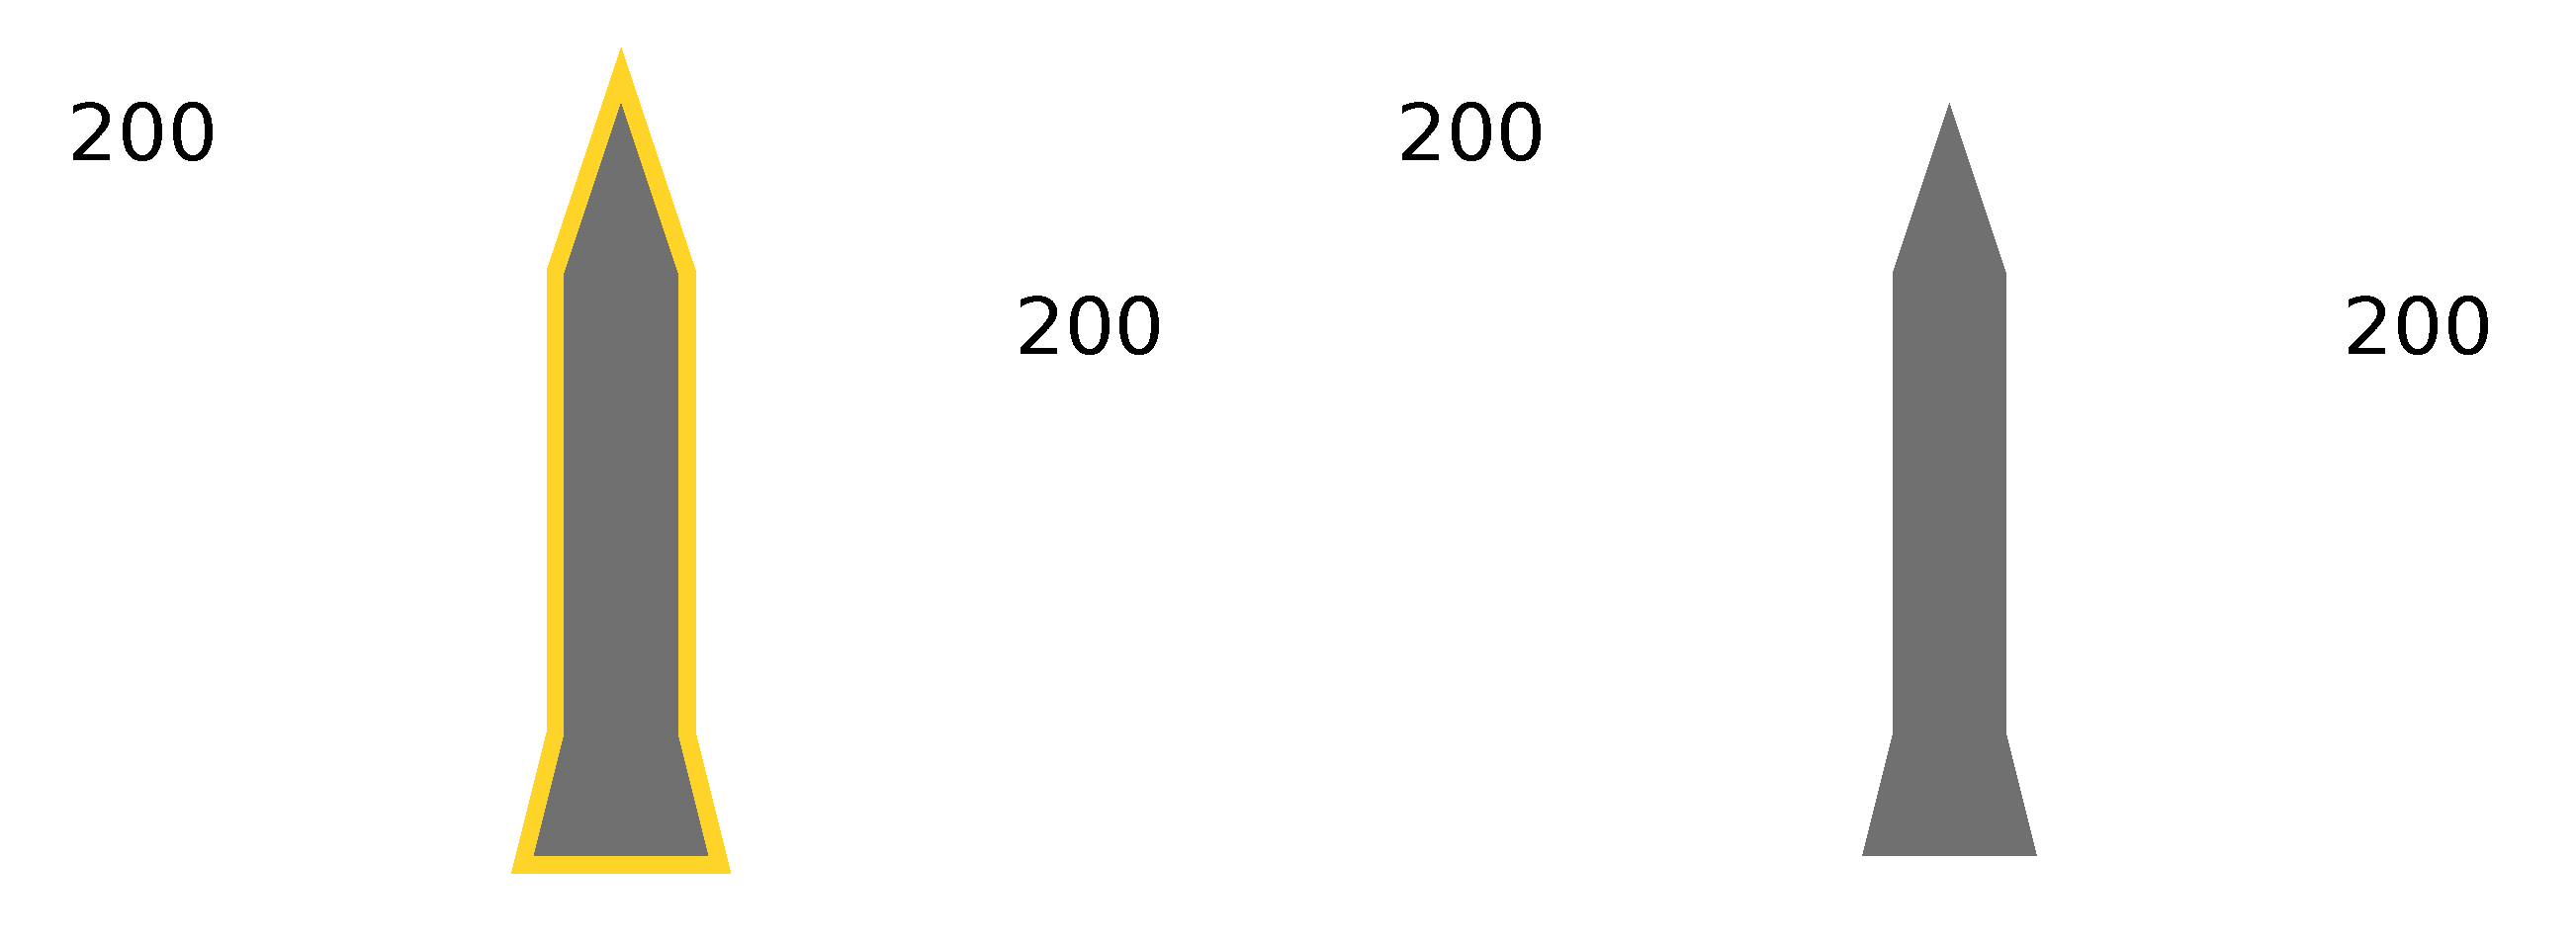
\includegraphics[width=0.8\textwidth]{images/zkp/measurement_step3.pdf}
\end{center}
\end{frame}

\begin{frame}[label=sec-5-7]{Detectors}
\begin{center}
Detectors could be Non-Electronic Devices
\end{center}

\begin{varblock}[\textwidth]{}
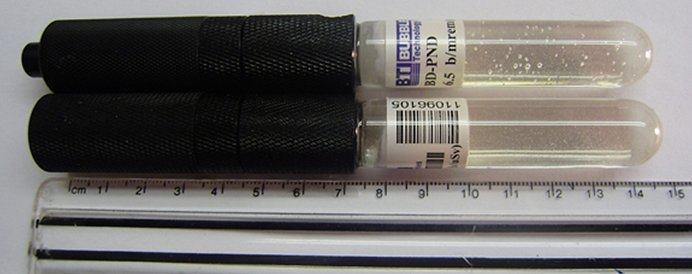
\includegraphics[width=\textwidth]{images/zkp/715781main_vial_XL.jpg}
\end{varblock}

\vspace{-0.7cm}
\tiny \textcolor{gray}{Public Domain - NASA}
\end{frame}

\begin{frame}[label=sec-5-8]{Current Research}
\footnotesize 

A. Glaser, B. Barak and R. J. Goldston, "A New Approach to Nuclear Warhead Verification Using a Zero-Knowledge Protocol", Proceedings of 53rd Annual INMM Meeting, Institute of Nuclear Materials Management, Orlando, Florida, July 15–19, 2012.\\[0.3em]

A. Glaser, B. Barak and R. J. Goldston. "A zero-knowledge protocol for nuclear warhead verification",  \emph{Nature}, 2014, 510, 497-502.\\[0.3em]



\pause

\vspace{1cm}

\begin{center}
\emph{Can you imagine to help?}
\end{center}
\end{frame}

\section{Conclusion}
\label{sec-6}

\begin{frame}[label=sec-6-1]{Summary}
\begin{center}
Nuclear Disarmament has relation to computers \& technology.
\end{center}
\pause

\begin{columns}[t]

\begin{column}{0.35\textwidth}

\tcbset{blackheight/.style={tcbeamer,valign=center,equal height group=blacks,notitle,colframe=black,colback=black}}
\begin{tcolorbox}[blackheight]
\tiny
\ttfamily
\textcolor{white}{while(totalnukes > 0) \{}

\hspace{0.3cm} \textcolor{white}{for(i=1; i<=9; i++) \{}

\hspace{0.6cm} \textcolor{white}{weaponstate[i]->disarm();}

\hspace{0.3cm} \textcolor{white}{\}}

\textcolor{white}{\}}
\end{tcolorbox}

\pause
\end{column}

\begin{column}{0.3\textwidth}
\tcbset{blackheight/.style={tcbeamer,valign=center,center upper,equal height group=blacks,notitle,colframe=black,colback=black}}
\begin{tcolorbox}[blackheight]

\includegraphics[width=\textwidth]{images/ib/ib_good}
\end{tcolorbox}

\pause
\end{column}

\begin{column}{0.3\textwidth}
\tcbset{blackheight/.style={tcbeamer,valign=center,center upper,equal height group=blacks,notitle,colframe=white,colback=black}}
\begin{tcolorbox}[blackheight]
    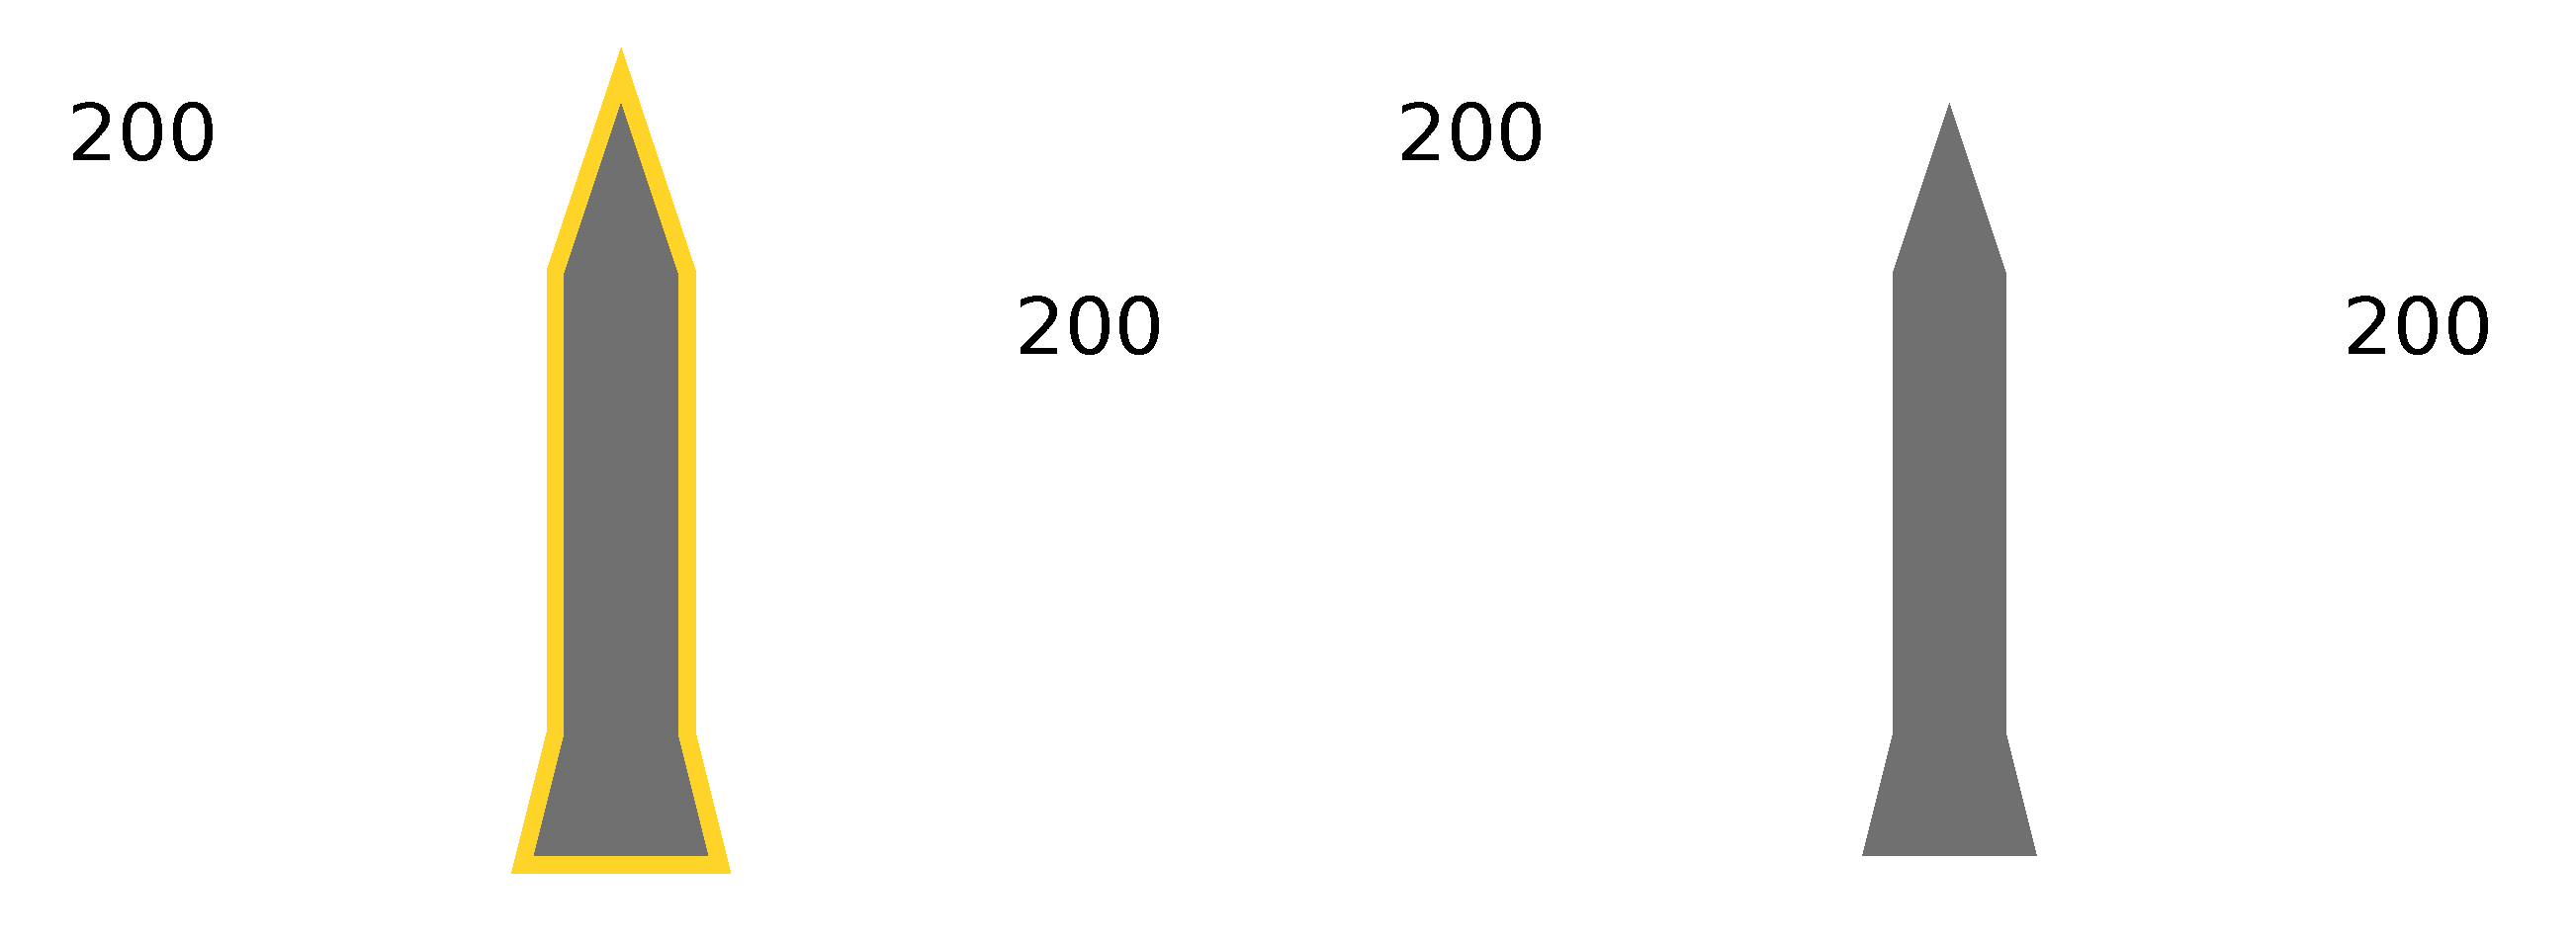
\includegraphics[width=\textwidth]{images/zkp/measurement_step3}
\end{tcolorbox}

\pause

\vspace{0.5cm}
\end{column}
\end{columns}

\begin{block}{Not the only tasks}
\small
\begin{itemize}
\item Virtual Reality for Training / Testing
\item Large Sensor Networks
\item Whistleblowing
\item \ldots{}
\end{itemize}
\end{block}
\end{frame}

\begin{frame}[label=sec-6-2]{}

\begin{center}
\Large
Thanks for listening!\\[1.5em]
\normalsize
Contact: moritz@nuclearfreesoftware.org\\[2em]
(and other: ZNF Hamburg, FIfF, local groups...)
\end{center}
\end{frame}


\appendix

\begin{frame}[label=sec-7-1]{Image References 1}
\fontsize{3pt}{3.6}\selectfont

\textcolor{gray}{In order of appearance, own work not listed}\\[0.5em]

CC-BY-SA Nanking2012 (Arak reactor): Creative Commons-Attribution-Share Alike, Nanking 2012, \url{http://commons.wikimedia.org/wiki/File:Arak_Heavy_Water4.JPG}, downloaded 2014-07-16 \\[0.3em]

CC-BY-SA Stefan-XP / Wikimedia Commons (Nuclear Fission): http://commons.wikimedia.org/wiki/File:Kernspaltung.svg, downloaded 2014-08-29 \\[0.3em]

CC-BY-SA Wikimedia Commons (Nuclear chain reaction): http://commons.wikimedia.org/wiki/File:Kettenreaktion.svg, downloaded 2014-08-29\\[0.3em]

Public Domain / Wikimedia Commons - modified (Gun-type weapon): \url{http://en.wikipedia.org/wiki/File:Fission_bomb_assembly_methods.svg}, downloaded 2014-08-18\\[0.3em]

Public Domain / Wikimedia Commons - modified (Implosion type weapon): \url{http://en.wikipedia.org/wiki/File:Implosion_nuclear_weapon_design_-_shock_waves.svg}, downloaded 2014-08-29\\[0.3em]

CC-BY-SA Sajak (AfE Tower Blasting), Sven-Sebastian Sajak, \url{http://upload.wikimedia.org/wikipedia/commons/2/23/140202_Afe-Tower_Blasting.jpg}, downloaded 2014-08-25\\[0.3em]

CC-BY-SA Robock et. al 2007 (Nuclear Winter), Robock, A.; Oman, L.; Stenchikov, G. L.; Toon, O. B.; Bardeen, C. and Turco, R. P. Climatic consequences of regional nuclear conflicts - Figure 5 Atmospheric Chemistry and Physics, 2007, 7, 2003-2012. (\url{http://www.atmos-chem-phys.net/7/2003/2007/}, downloaded 2014-08-28).\\[0.3em]

CC-BY-SA Stahlkocher (Airbase Büchel), \url{http://commons.wikimedia.org/wiki/File:B\%C3\%BCchel_Fliegerhorst.jpg}, downloaded 2014-09-01.\\[0.3em]

Public Domain, U.S. DoD (B61 bombs), United States Department of Defense (SSGT Phil Schmitten), \url{http://de.wikipedia.org/wiki/Datei:B-61_bomb_rack.jpg}, downloaded 2014-08-22.\\[0.3em]

CC-BY-NC IPFM, Global Fissile Material Report 2009, International Panel on Fissile Materials, Princeton, 2009, p. 67.\\[0.3em]
\end{frame}

\begin{frame}[label=sec-7-2]{Image References 2}
\fontsize{3pt}{3.6}\selectfont

Public Domain - FSF (Free Software Foundation Logo), \url{http://commons.wikimedia.org/wiki/File:Free_Software_Foundation_logo_and_wordmark.svg}, downloaded 2014-07-07.\\[0.3em]

CC-BY-SA NicoBZH (portrait of Richard Stallman), NicoBZH from Saint Etienne - Loire, France, \url{http://commons.wikimedia.org/wiki/File:NicoBZH_-_Richard_Stallman_\%28by-sa\%29_\%285\%29.jpg}, downloaded 2014-07-07.\\[0.3em]

CC-BY Open Source Initiative (OSI Logo), \url{http://commons.wikimedia.org/wiki/File:Opensource.svg}, downloaded 2014-07-07.\\[0.3em]

CC-BY-SA Manon Anne Ress (portrait of Bruce Perens): \url{http://commons.wikimedia.org/wiki/File:Bruce_perens_13jan09_tacd_MAR_1557x1188.JPG}, downloaded 2014-07-07.\\[0.3em]

Public Domain - U.S. DoE NNSA (Warhead Measurement Campaing), U.S. Department of Energy - National Nuclear Security Administration, \url{http://nnsa.energy.gov/sites/default/files/imagecache/feature_photo_689w_249h/nnsa/09-13-featurephoto/2013-09-30\%20na22\%203\%20topline.PNG}, downloaded 2014-09-01.\\[0.3em]

CC-BY-SA Cowjuice - Wikimedia Commons (Raspberry Pi), \url{http://commons.wikimedia.org/wiki/File:Raspberry_Pi_Photo.jpg}, downloaded 2014-09-01.\\[0.3em]


Public Domain - NASA (Bubble Detectors), \url{http://www.nasa.gov/images/content/715781main_vial_XL.jpg}, downloaded 2014-08-29.\\[0.3em]
\end{frame}




\begin{frame}[label=sec-7-3]{}

\end{frame}

\begin{frame}[label=sec-7-4]{Effects of a nuclear explosion}
\begin{alertblock}{Thermal radiation}

"Spontaneous" ignition of items, firestorm, burns.
\end{alertblock}

\begin{alertblock}{Blast / pressure wave}

Destruction of buildings and debris production.

Similar to conventional weapons, but more intense.
\end{alertblock}

\begin{alertblock}{Radiation (direct / indirect)}
Direct radiation from neutron / gamma emitted in reaction.

Indirect radiation (later) from activated debris.
\end{alertblock}
\end{frame}

\begin{frame}[label=sec-7-5]{Effects of nuclear weapons}
\begin{center}
Footage:

US test series: Upshot-Knothole

March 17, 1953

Explosion Annie (on tower)
\end{center}

\begin{tikzpicture}[remember picture,overlay]
    {{\uncover<2->{\node [line width=1mm, draw=black, inner sep=0pt] at (current page.center) {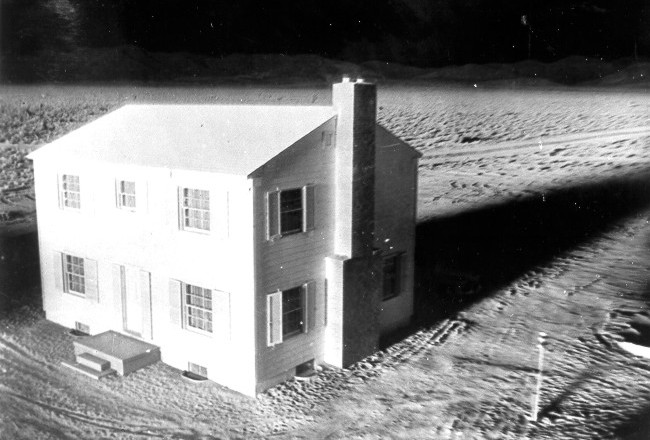
\includegraphics[width=12cm]{images/upshot_knothole/01.jpg}};}}};
    {{\uncover<3->{\node [line width=1mm, draw=black,inner sep=0pt] at (current page.center) {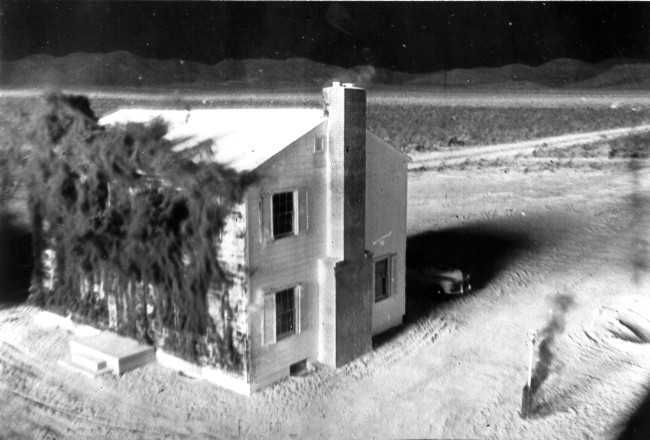
\includegraphics[width=12cm]{images/upshot_knothole/02.jpg}};}}};
    {{\uncover<4->{\node [line width=1mm, draw=black,inner sep=0pt] at (current page.center) {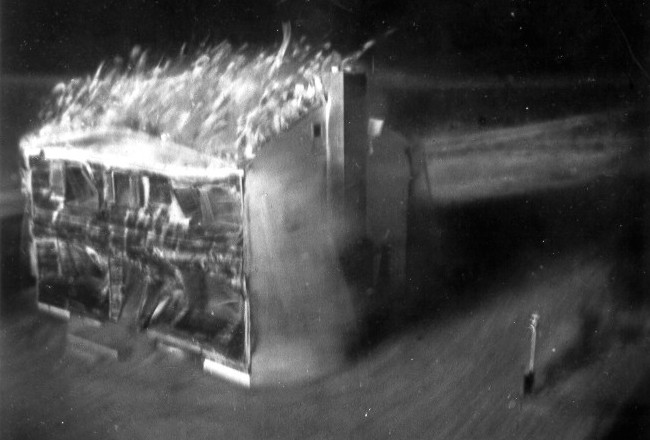
\includegraphics[width=12cm]{images/upshot_knothole/03.jpg}};}}};
    {{\uncover<5->{\node [line width=1mm, draw=black,inner sep=0pt] at (current page.center) {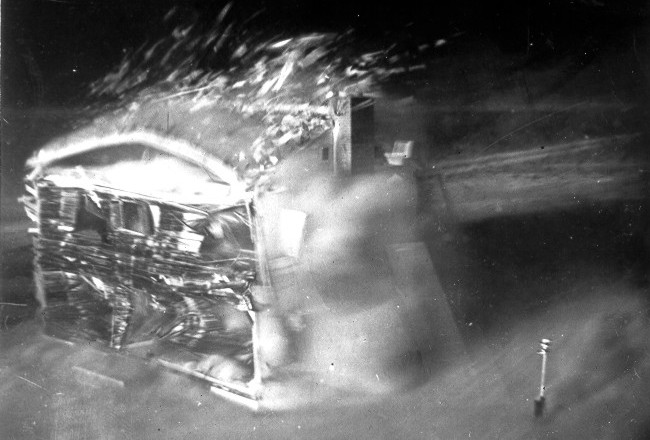
\includegraphics[width=12cm]{images/upshot_knothole/04.jpg}};}}};
    {{\uncover<6->{\node [line width=1mm, draw=black,inner sep=0pt] at (current page.center) {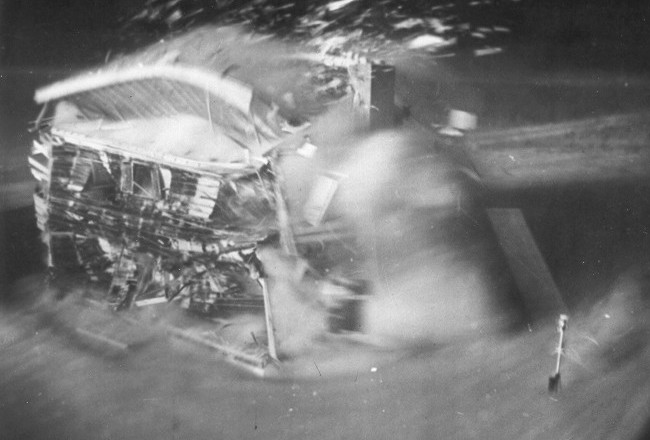
\includegraphics[width=12cm]{images/upshot_knothole/05.jpg}};}}};
    {{\uncover<7->{\node [line width=1mm, draw=black,inner sep=0pt] at (current page.center) {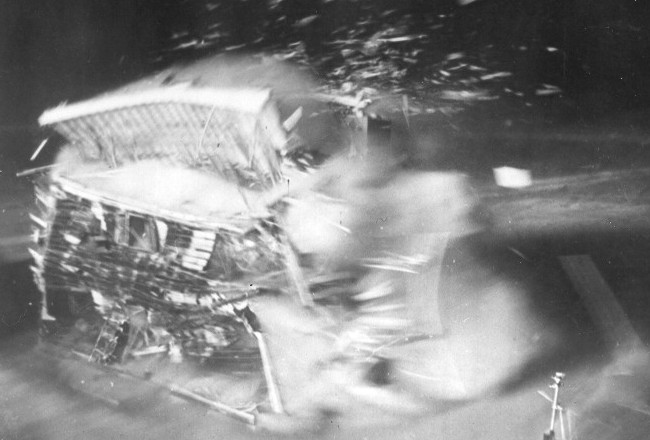
\includegraphics[width=12cm]{images/upshot_knothole/06.jpg}};}}};
    {{\uncover<8->{\node [line width=1mm, draw=black,inner sep=0pt] at (current page.center) {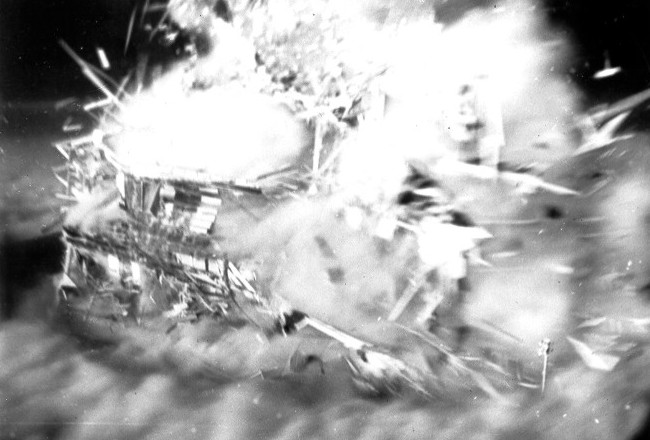
\includegraphics[width=12cm]{images/upshot_knothole/07.jpg}};}}};
    {{\uncover<9->{\node [line width=1mm, draw=black,inner sep=0pt] at (current page.center) {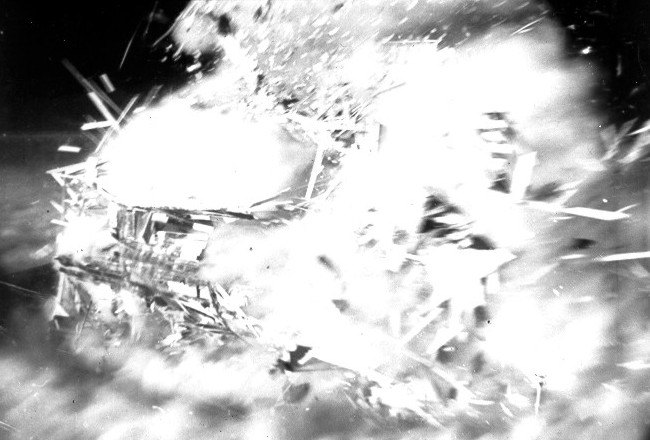
\includegraphics[width=12cm]{images/upshot_knothole/08.jpg}};}}};
   {{\uncover<2->{\node [shift={(-3.3cm, -3.8cm)}, fill=white, line width=1mm, draw=white,inner sep=0pt] at (current page.center) {\tiny \textcolor{gray}{Public Domain, U.S. DoE - Nevada Field Office}};}}};
\end{tikzpicture}
\end{frame}


\begin{frame}[label=sec-7-6]{Examples for Software Use}

\begin{table}[htb]
\fontsize{7pt}{8.4}\selectfont
\begin{center}
\begin{tabularx}{\textwidth}{>{\bf}RLLLL}
\toprule
  & \bf Non-Proliferation / Safeguards  & \bf Fissile Material Cutoff Treaty  & \bf Nuclear Disarmament Agreement  \\
\toprule
 Particle Transport (Stochastic/ Deterministic) & Development of NDA methods for fresh/spent fuel analysis & Development of NDA methods for material analysis   & Development of NDA methods for warhead authentication \\
\midrule
 Depletion Calculations & Proliferation potential of reactors  & Estimate past/current fissile material production capabilities & Fission product tagging for warhead identification \\
\midrule
 Spectrum Analysis & Identify items (spent/fresh fuel), determine material compositions & Identify items (spent/fresh fuel), determine material compositions & Identify items (warheads) and respective material compositions \\
% \midrule
%  Correlation Analysis & Neutron Correlation/Multiplicity measurements for Pu-mass estimates &  &   & Neutron Correlation/Multiplicity Measurements for Pu-mass estimates \\
% \midrule
%  Atmospheric Transport Modeling & Kr-85 detection (clandestine reprocessing) & Radionuclide detection & Kr-85 detection  &   \\
% \midrule
% Fuel Cycle Simulation & Material Balancing and Accounting & & Material Balancing \& Accounting, Past Fissile Material Production &  \\
% \midrule
% Fluid Dynamics & Isotope Separation Modeling & Enrichment Cascade Analysis & & Nuclear Archaeology  \\
%  Waveform Analysis &   & Discriminate Explosion and Earthquake &   &   \\
% \midrule
%  Image Identification & Find clandestine facilities  &  & Finding clandestine facilities  &   \\
% \midrule
%  Image Change Detection & Find clandestine facilities, track operational status of existing ones & Detect crater / sinkings after explosions & check operational status of facilities  & Warhead Chain-of-custody  \\
% \midrule
%  Geographic Information System & Combine data from different sources  & Reconstruct possible locations of explosions &   &   \\
% \midrule
% Virtual Realities & Inspector Training, Data visualization & Training for On-Site Inspections & & Improvement of verification process \\
% \midrule
%  General Purpose Data Analysis & Visualize/edit complex data-sets  & Visualize/edit complex data-sets & Visualize/edit complex data-sets  & Visualize/edit complex data-sets  \\
\bottomrule
\end{tabularx}
\end{center}
\label{tab:fields}
\end{table}

\begin{center}
\textcolor{gray!50}{\scriptsize (Extensive table in M. Kütt, A. Glaser, M. Englert: Open Source meets Nuclear Arms Control, in proceedings of 55th Annual INMM Meeting, Atlanta, GA, 21-24 July 2014)}
\end{center}
\end{frame}

\begin{frame}[label=sec-7-7]{Safecast}
\vspace{-0.5cm}
\begin{columns}
\begin{column}{0.4\textwidth}
\begin{varblock}[\textwidth]{}
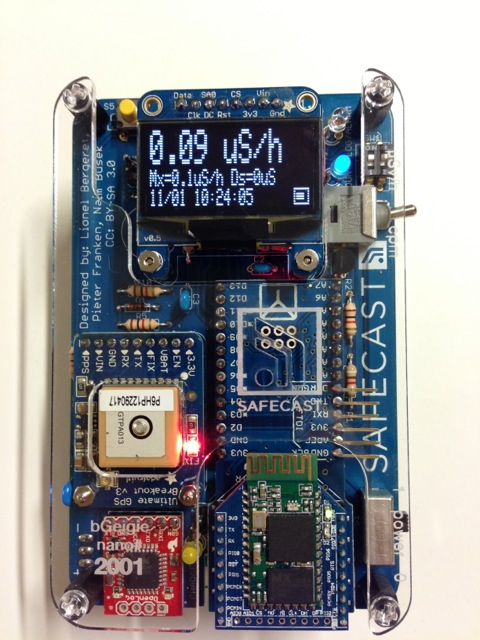
\includegraphics[width=\textwidth]{images/bgeigie_IMG_0009.jpeg}\\
bGeigie nano
\end{varblock}
\vspace{-0.3cm}
\tiny \textcolor{gray}{CC-BY Safecast}
\end{column}

\begin{column}{0.4\textwidth}
\begin{varblock}[\textwidth]{}
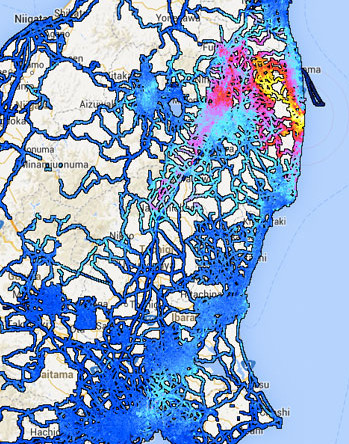
\includegraphics[width=\textwidth]{images/safecast_japan_crop.jpg}\\
Measurements in Japan
\end{varblock}
\vspace{-0.3cm}
\tiny \textcolor{gray}{CC-BY Safecast}
\end{column}
\end{columns}
\end{frame}


\begin{frame}[label=sec-7-8]{Appendix Image References}
\fontsize{3pt}{3.6}\selectfont

Public Domain - U.S. DoE Nevada Field Office (Test Upshot-Knothole), \url{http://www.nv.doe.gov/library/photos/upshot.aspx}, downloaded 2013-08-10.\\[0.3em]

CC-BY Safecast (bGeigie nano): Creative Commons-Attribution, Safecast Project, \url{http://blog.safecast.org/wp-content/uploads/2013/03/IMG_0009.jpeg}, downloaded 2014-07-25.\\[0.3em]

CC-BY Safecast (Japan Map): Creative Commons-Attribution, Safecast Project, \url{http://blog.safecast.org/wp-content/uploads/2014/05/980x480.jpg}, downloaded 2014-07-25 (cutout).\\[0.3em]
\end{frame}
\begin{frame}[label=sec-7-9]{}

\begin{center}

\includegraphics[width=0.2\textwidth]{by-nc-sa_eu.png}

This work is licensed under the Creative Commons Attribution-NonCommercial-ShareAlike 4.0 International License. To view a copy of this license, visit \url{http://creativecommons.org/licenses/by-nc-sa/4.0/}.
\end{center}
\end{frame}
% Emacs 24.3.1 (Org mode 8.2.7b)
\end{document}
